% !TeX spellcheck = en_GB
\PassOptionsToPackage{square,comma,numbers,sort&compress}{natbib}

\documentclass{article}

\usepackage[preprint]{neurips_2019}

\usepackage{easyReview}
\usepackage[utf8]{inputenc} % allow utf-8 input
\usepackage[T1]{fontenc}      % use 8-bit T1 fonts
\usepackage{hyperref}      		 % hyperlinks
\usepackage{url}            			% simple URL typesetting
\usepackage{nicefrac}      		  % compact symbols for 1/2, etc.
\usepackage{microtype}     		% microtypography
\usepackage[inline]{enumitem}
\usepackage{amsmath}
\usepackage{amsfonts}       	 % blackboard math symbols
\usepackage{mathtools} 
\usepackage {xcolor}
%\usepackage[section]{placeins} % Prevent figures from being moved across sections
% Reset subcaption counters at the start of figure/table float
\usepackage{subcaption}
\usepackage{tabularx}
\usepackage{bm}
\usepackage{mathtools} 
\usepackage{longtable, booktabs}
\usepackage{makecell}
\usepackage{multirow}
\usepackage{diagbox}
\usepackage{latexsym}
\usepackage{stmaryrd}
\usepackage{siunitx}
\def\tabularxcolumn#1{m{#1}}
\usepackage{graphicx}
\graphicspath{ {images/} }

\title{GANsformer Reproducibility Challenge}

\author{%
Giorgia Adorni \\
\texttt{giorgia.adorni@usi.ch} \\
\And
Felix Boelter\\
\texttt{felix.boelter@usi.ch}\\
\And
Stefano Carlo Lambertenghi\\
\texttt{stefano.carlo.lambertenghi@usi.ch}\\
}

\begin{document}

\maketitle
\begin{abstract}
	The field of image generation through generative modelling is abundantly discussed nowadays. It 
	can be used for a highly varied range of applications such as up-scaling 
	already existing images, creating non-existing objects, such as interior design scenes,
	products or even human faces, and achieving transfer-learning processes. 
	In this context, Generative Adversarial Networks (GANs) are a class of widely studied machine 
	learning frameworks first appearing in the paper ``\emph{Generative adversarial nets}'' by 
	\citet{goodfellow2014generative} that achieve the aforementioned goal. 
	In our work, we reproduce and evaluate a novel variation of the original GAN network, the 
	GANformer, proposed in ``\emph{Generative adversarial Transformers}'' by 
	\citet{hudson2021generative}. 
	The goal of this project was to recreate the methods presented by this paper to reproduce the 
	original results and comment on the authors’ claims. 
	Due to resources and time limitations, we had to constraint the networks training times and 
	dataset types and sizes. 
	Our research successfully recreated both variations of the proposed GANformer model and found 
	extreme differences between the authors’ and our results. 
	Moreover, discrepancies between the publication methodology and the one implemented, 
	made available in the code, allowed us to study two undisclosed variations of the presented 
	procedures.
\end{abstract}

\section{Introduction}
This project aims at investigating the reliability and reproducibility of a paper accepted 
for publication in a top machine learning conference. The models have been implemented 
using code and information provided by the authors.

With this work, we are going to verify the empirical results and claims of the paper 
``\emph{Generative adversarial Transformers}'' by \citet{hudson2021generative}, by reproducing 
three of the computational experiments performed by the authors:
\begin{enumerate*}
	\item[(1)] the \textit{StyleGAN2} by \citet{karras2020analyzing,karras2019style}, a GAN 
	network that uses one global latent style vector to modulate the features of each layer, hence 
	controlling the style of all image features globally.
	\item[(2)] the \textit{GANformer} with \textit{Simplex Attention} by 
	\citet{hudson2021generative}, which generalises the StyleGAN design with \textit{k} latent 
	vectors that cooperate through attention. Thus, allowing for a spatially finer control over the 
	generation 
	process since multiple style vectors impact different regions in the image concurrently, 
	particularly 
	permitting communication in one direction, in the generative context – from the latent vectors to 
	the 
	image features.
	\item[(3)] the \textit{GANformer} with \textit{Duplex Attention} by \citet{hudson2021generative}, 
	which is based on the same principles as the previous but propagating information from 
	global latent vectors to local image features, enabling both top-down and bottom-up reasoning to 
	coincide.
\end{enumerate*} 

The first model is used as a baseline, while the remaining are the architectures introduced by the 
authors. 
They consider the GANformer as “a novel and efficient type of transformer” which demonstrates its 
strength 
and robustness over a range of tasks of visual generative modelling — simulated multi-object 
environments 
(real-world indoor and outdoor scenes) — achieving state-of-the-art results in terms of both image 
quality 
and diversity while benefiting from fast learning and better data-efficiency.

\section{Background}\label{sec:background}
\subsection{Generative Adversarial Networks (GANs)}\label{sec:gan}
Generative Adversarial Networks (GANs) \cite{goodfellow2014generative} are deep-learning-based 
generative models which learn to determine whether a sample is from the model or the data 
distribution. 
The classic architecture, illustrated in Appendix \ref{subsec:app_background} in Figure 
\ref{fig:gan}, is 
composed by two main neural networks: 
the \textit{generator} ${G(z)}$, which generates new plausible examples in the problem domain — 
images in our case — , and the \textit{discriminator} ${D(x)}$, which classify the examples as 
real (coming from the training dataset) or fake (generated by $G$). 
%	More details are provided in Appendix \ref{subsec:app_background}.

\subsection{StyleGAN2}\label{sec:StyleGAN}
StyleGANs are a re-design of the GANs generator architecture, which aim is to control the image 
synthesis process \cite{karras2019style}. The typical architecture of a StyleGAN is shown in 
%	Appendix \ref{subsec:app_background} in Figure \ref{fig:StyleGAN}, together with the technical 
%	details. 

In particular, we are interested in the second version of the StyleGAN, the StyleGAN2 
\cite{karras2020analyzing}, which is a revisiting of the architecture of the StyleGAN synthesis 
network. 
%	Figure \ref{fig:StyleGAN2} in Appendix \ref{subsec:app_background} exemplifies the 
%	various changes made to the original architecture up to the final StyleGAN2 network. Further 
%	information is provided in Appendix \ref{subsec:app_background}.

The StyleGAN2 architecture makes it possible to control the image synthesis via scale-specific 
modifications to the styles. In particular, this approach attains layer-wise decomposition of visual 
properties, allowing StyleGAN to control global aspects of the picture such as pose, lighting 
conditions or colour schemes, in a coherent manner over the entire image.

However, while this model successfully disentangles global properties, it is more limited in its ability to perform spatial decomposition, as it provides no direct means to control the style of a localised 
regions within the generated image.

\subsection{Transformers}\label{sec:transformer}
Transformers are deep-learning models based on an \textit{attention mechanism}, which is 
designed 
to handle sequential input data and evaluate the relationship between each input-output item 
\cite{vaswani2017attention}.
This model, unlike Recurrent Neural Networks (RNNs), avoids using convolutions or aligned 
sequences, and do not necessarily require ordered input data to be processed. 
The architecture is composed by an \textit{encoder-decoder} structure where, the {encoder} maps 
an input sequence of symbol representations $(x_1,\dots, x_n)$ to a sequence of continuous 
representations $z = (z_1, \dots, z_n)$, while the  {decoder}, given $z$, generates an output 
sequence $(y_1, \dots, y_m)$ of symbols one element at a time. 
Each transformer module (encoder-decoder) is connected to each other via feed-forward
layers.

%	The details about how an attention function works are reported in Appendix 
%	\ref{subsec:app_background}. 

\citet{vaswani2017attention}used multiple multi-head attentions stacked on top of each other, 
enabling to pass multiple input sequences simultaneously, instead of one at a time, allowing for 
more parallelisation and reducing training times if one has access to sufficient computational 
resources.

\section{Methodology: Generative Adversarial Transformers}\label{sec:ganformer}
%	In this section you should give a description of the methodological aspects of your work, for 
%	instance how you modified an existing method to perform a particular task or to overcome a 
%	particular limitation. If your project is about reproducibility, here you should describe the method 
%	presented in the original paper.

The Generative Adversarial Transformers (GANsformer), introduced by 
\citet{hudson2021generative}, are models which combine GANs and the transformers to 
generate 
better and more realistic examples.

GANs, and in particular the StyleGAN2 model \cite{karras2020analyzing}, presented in Section 
\ref{sec:StyleGAN}, %and shown in Figure \ref{fig:StyleGAN2}, 
is used as a starting point for the 
GANformer design for the properties it owns as CNN: they are powerful generators for the overall 
style of the image, since by nature they merge the local information of the pixels together with the 
general information regarding the image. 
However, they are less powerful with respect to small details of localised regions within the 
generate 
image itself, since they miss out on the long range interaction of the faraway pixel.

Accordingly, GANsformers take advantage of the transformers attention mechanism to make the 
StyleGAN2 architecture even more powerful: the integration of attention in the architecture allows 
the network to draw global dependencies between input and output, and understand the context of 
the image thanks to the transformer's strength for long-range interactions.
Thus, rather than focusing on using global information and controlling all features globally, 
the transformer uses attention to propagate information from the local pixels to the global high-level 
representation and vice versa. 

The \textit{bipartite transformer} structure computes \textit{soft attention}, iteratively aggregating 
and disseminating information between the generated image features and a compact set of 
\textit{latent variables} enabling bidirectional interaction between these dual representations. 
This architecture offers a solution to the StyleGAN limitation in its ability to perform spatial 
decomposition which leads to the impossibility of controlling the style of a localised region 
within the generated image.
%	More details regarding the composition and functioning of the bipartite transformer and 
%	self-attention layers are thorough in Appendix \ref{subsec:app_methodology}. 

The \textit{transformer network} corresponds to the \textit{multi-layer bidirectional transformer 
	encoder} (BERT), introduced by \citet{devlin2019bert}, which interleaves \textit{multi-head 
	self-attention} and \textit{feed-forward layers}. 

The discriminator model performs multiple layers of convolution down-sampling on the image, 
reducing the representation's resolution gradually until making final prediction. 
Optionally, attention can be incorporated into the discriminator as well where it has multiple $k$ 
aggregator variables, that use attention to adaptively collect information from the image while being 
processed. 

The generator likewise is composed of two parts, a mapping network and a synthesis 
network. 
The mapping network of a GANformer is the same as that of the StyleGAN2.
In the synthesis network, while in the StyleGAN2, a single global $w$ vector controls all the 
features equally, the GANformer uses attention so that the $k$ latent components specialise to 
control different regions in the image to create it cooperatively, and therefore perform better 
especially in generating images depicting multi-object scenes, also allowing for a flexible and 
dynamic style modulation at the region level.

\citet{hudson2021generative} have applied some adaptations to the structure of the GANformer as 
presented here, in order to foster an interesting communication flow. The details are provided later 
in Section \ref{sec:hyperparam}.
Rather than densely modelling interactions among all the pairs of pixels in the images, instead it 
supports \textit{adaptive long-range interaction} between far away pixels in a moderated manner, 
passing through a compact and global latent bottleneck that selectively gathers information from 
the entire input and distributes it back to the relevant regions. 

There are two attention operations that could be computed over the bipartite graph, depending 
on the direction in which information propagates, 
\begin{enumerate*}
	\item [(1)] \textit{simplex attention} permits communication either in one way only, in the 
	generative context, from the latent vectors to the image features, and
	\item [(2)] \textit{duplex attention}, which enables it both top-down and bottom-up.
\end{enumerate*}

\subsection{Simplex attention}
\comment{The simplex and duplex attention layers and formulas are provided in the original article}{I'm not sure about keeping all the details regarding simplex and duplex attention since we can find these stuff exactly the same in the original paper. }
As already mentioned, simplex attention distributes information in a single direction over the 
bipartite transformer graph. 

Formally, let $X^{n\times d}$ denote an input set of $n$ vectors of dimension $d$ — where, for the 
image case, $n = W\times H$ — and $Y^{m\times d}$ denote a set of $m$ aggregator variables — 
the latent variables, in the generative case. Specifically, the attention is computed over the derived 
bipartite 
graph between these two groups of elements, as in Equation \eqref{eqn:attention}, moreover:
\begin{equation}
	\label{eqn:attention2}
	a(X,Y)=\mathsf{Attention}(q(X), k(Y), v(Y)) \mbox{,}
\end{equation}
where $q(\cdot), k(\cdot), v(\cdot)$ are functions that respectively map elements into queries, 
keys, and values, all maintaining dimensionality $d$. 
The mappings are provided with positional encodings to reflect the distinct position of each element 
(e.g. in the image). This bipartite attention is a generalisation of self-attention, where $Y = X$.

Standard transformers implement an additive update rule of the form:
\begin{equation}
	\label{eqn:layernorm}
	u^a(X, Y)=\mathsf{LayerNorm}(X + a(X, Y)) \mbox{,}
\end{equation}
however, \cite{hudson2021generative} used the retrieved information to control both the scale as 
well as the bias of the elements in $X$, in line with the practice promoted by the StyleGAN model 
\cite{karras2019style}:
\begin{equation}
	\label{eqn:simplex}
	u^s(X, Y)=\gamma (a(X, Y)) \odot \omega (X) + \beta (a(X, Y)) \mbox{,}
\end{equation}
where $\gamma(\cdot), \beta(\cdot)$ are mappings that compute multiplicative and additive styles 
(gain and bias), maintaining dimensionality $d$, and $\omega (X) = X- \mu(X)$ normalises each 
element with $\sigma(X)$ respect to the other features. By normalising $X$ (image features), and 
then letting $Y$ (latent vectors) control the statistical tendencies of $X$, the information 
propagation from 
$Y$ to $X$ is enabled, allowing the latent vectors to control the visual generation of spatial 
attended 
regions within the image, so as to guide the synthesis of objects or entities.
The multiplicative integration permits significant gains in the model performance. 

\subsection{Duplex attention}
Duplex attention can be explained by taking into account the variables $Y$ to set their own 
key-value structure: $Y = (K^{n\times d} , V^{n\times d})$, where the values store the content of the 
$Y$ variables, as before (e.g. the randomly sampled latent vectors in the case of GANs) while the 
keys track the centroids $K$ of the attention-based assignments between $Y$ and $X$, which can 
be computed as $K = a(Y, X)$ — namely, the weighted averages of the $X$ elements using the 
bipartite attention distribution derived through comparing it to $Y$. 
Consequently, the new update rule is defined as follows:
\begin{equation}
	\label{eqn:duplex}
	u^d(X, Y )=\gamma (A(X, K, V)) \odot \omega (X) + \beta (A(X, K, V)) \mbox{,}
\end{equation}
where, two attention operations are compound on top of each other: first compute the \textit{soft 
	attention} assignments between $X$ and $Y$, by $K = a(Y, X)$, and then refine the assignments 
by 
considering their centroids, by $A(X, K, V)$. This is analogous to the \textit{k-means algorithm} and 
works more effectively than the simpler update $u^a$ defined above in Equation \eqref{eqn:simplex}.

Finally, to support bidirectional interaction between $X$ and $Y$ (the image and the latent vectors), 
two 
reciprocal simplex attentions are chained from $X$ to $Y$ and from $Y$ to $X$, obtaining the 
duplex 
attention, which alternates computing $Y :=u^a(Y,X)$ and $X:=u^d(X,Y)$, such that each 
representation is refined in light of its interaction with the other, integrating together bottom-up and 
top-down interactions.

\section{Implementation}
\comment{}{All this section should be revised since we are using also another dataset}
The code from the authors' has been merged with the code provided by StyleGAN2 to obtain a 
hybrid version of the StyleGAN2 and the GANformer. In addition, we created a simplified version of the code which removed unnecessary operations in the creation of the network that were used for other model architectures. Furthermore, we implemented a Google Colab Pro version of the authors’ code, as we had access to a more powerful GPU.

\subsection{Datasets}	\label{sec:dataset}
The original paper \cite{hudson2021generative} explored the GANformer model on four datasets for 
images and scenes: CLEVR \cite{johnson2017clevr}, LSUN-Bedrooms \cite{yu2015lsun}, Cityscapes 
\cite{cordts2016cityscapes} and FFHQ \cite{karras2019style}. 

Initially, we used the Cityscapes dataset since it is smaller among the four: it contains 
25k images with 256x256 resolution. 
However, the memory required to complete the training was too high on this dataset (more than 
25Gb).
Even if we had more memory available, Colab Pro's limitation of 24 hours sessions would have 
interrupted our experiments prematurely.

For this reason, we switch to another dataset, the Google Cartoon Set \cite{cartoonset}\footnote{	
	\url{https://google.github.io/cartoonset}}, containing 10k 2D cartoon avatar 
images with 64x64 resolution, composed of 16 components that vary in 10 artwork attributes, 4 
colour attributes, and 4 proportion attributes (see Table \ref{tab:dataset} in Appendix 
\ref{sec:cartoon-results}). 

After an initial examination of the result obtained with this dataset, we decided to proceed further using a more challenging dataset, the FFHQ, exploited in fact from the authors of the reproduced paper. 
This dataset, presented by \citet{karras2019style}, is a collection 70k high-quality images of human faces at a $1024×1024$ resolution, meaning that it offers a much higher quality and a vastly more variation in terms of age, ethnicity, image background and coverage of accessories such as eyeglasses, sunglasses, hats, etc., than existing high-resolution datasets.
\comment{}{add information about the resolution that we choose and components maybe}


\subsection{Hyper-parameters and design choices}\label{sec:hyperparam}
In this section we present the relevant hyper-parameters used in our experimentation, both for 
training and also in terms of layer sizes and technical choices.

Table \ref{tab:hyper} contains a comparison between StyleGAN2 (the baseline) and the novel 
networks proposed in the original paper.

Note that in the code provided by the author \cite{hudson2021generative}, the 
hyper-parameters are not the same as mentioned in the article.

\newcolumntype{Y}{>{\raggedleft\arraybackslash}X}
\begin{table}[htb]
	\centering
	\caption{\textbf{Comparison of the hyper-parameters given in the code with those mentioned in 
			the paper statements}. $\mbox{GANformer}_{s}$ refers to the GANformer with Simplex 
			attention, 
		while $\mbox{GANformer}_{d}$ refers to the GANformer with duplex attention.}
	\label{tab:hyper}
	\vspace{3mm}
	\small
	\begin{tabularx}{\linewidth}{l|rYYYY}
		\toprule
		& \textbf{StyleGAN2} & \textbf{$\mbox{GANformer}_{s}$} (code) & 
		\textbf{$\mbox{GANformer}_{d}$} (code) & \textbf{$\mbox{GANformer}_{s}$}  (article) & 
		\textbf{$\mbox{GANformer}_{d}$} (article) \\
		\midrule
		\texttt{latent\_size}    & --    & 32   & 32    & 32    & 32 \\
		\texttt{dlatent\_size}   & --    & 32   & 32    & 32    & 32  \\
		\texttt{components\_num} & --    & 16   & 16    & 16    & 16   \\
		\texttt{beta1}           & 0.0   & 0.0  & 0.0   & 0.9   & 0.9  \\
		\texttt{beta2}           & 0.99  & 0.99 & 0.99  & 0.999 & 0.999  \\
		\texttt{epsilon}         & 1e-8  & 1e-8 & 1e-8 &  1e-3  & 1e-3 \\
		\bottomrule                                    
	\end{tabularx}
\end{table}

A \textit{kernel size} of $k = 3$ is used after each application of the attention, together with a 
\textit{Leaky ReLU non-linearity} after each convolution and then up-sample or down-sample the 
features $X$, as part of the generator or discriminator respectively, as in e.g. StyleGAN2 
\cite{karras2020analyzing}. 
To account for the features location within the image, we use a sinusoidal positional encoding along 
the horizontal and vertical dimensions for the visual features $X$, and trained positional 
embeddings for the set of latent variables $Y$.
Overall, the bipartite transformer is thus composed of a stack that alternates attention (simplex or 
duplex), convolution, and up-sampling layers, starting from a $4 \times 4$ grid up to the desirable 
resolution. 

Both the simplex and the duplex attention operations enjoy a bi-linear efficiency of 
$\mathcal{O}(mn)$ thanks to the network’s bipartite structure that considers all pairs of 
corresponding elements from $X$ and $Y$. Since, as we see below, we maintain $Y$ to be of a fairly 
small size, choosing m in the range of 8–32, this compares favourably to the prohibitive 	
$\mathcal{O}(n^2)$  complexity of self-attention, which impedes its applicability to high-resolution 
images.

As to the loss function, optimisation and training configurations, we adopt the settings and 
techniques used in StyleGAN2 \cite{karras2020analyzing}, including in particular style mixing, 
stochastic variation, exponential moving average for weights, and a non-saturating logistic loss with 
a lazy R1 regularisation.

\subsection{Experimental setup}	
The source code of our work is available at the following GitHub repository: 
\url{https://github.com/GiorgiaAuroraAdorni/gansformer-reproducibility-challenge}.

The approaches proposed in both the original paper codebase by \citet{karras2020analyzing} and 
by \citet{hudson2021generative} have been implemented in Python using TensorFlow 
\cite{tensorflow2015-whitepaper}, so, according to that, we used the same setup.
We created a Jupyter Notebook which runs all the experiments in Google Colaboratory, which 
allows us to write and execute Python in the browser. 

All the models have been trained on a Tesla P100-PCIE-16GB (GPU) provided by Google 
Colab Pro.

\subsection{Computational requirements}\label{sec:comput_req}

In the original paper \cite{hudson2021generative}, they evaluate all models under comparable 
conditions of training scheme, model size, and optimisation details, implementing all the models 
within the codebase introduced by the StyleGAN authors \cite{karras2020analyzing}. 
All models have been trained with images of 256 x 256 resolution and for the 
same number of training steps, roughly spanning a week on 2 NVIDIA V100 GPUs per model (or 
equivalently 3-4 days using 4 GPUs). 

Considered that we had available just one GPU and not enough time to reproduce this settings, we 
decided to resize the images from 256x256 to 64x64 resolution.


For the GANformer we select k = 32 number of latent variables. 

All models have been trained for the same number of steps, 300 000 image
training samples (300 kimg) while the paper present results after training 100, 200, 500, 1000, 2000, 
5000 and 10000 kimg samples

For the StyleGAN2 model we present results after training 300 kimg, obtaining 
good results.
Note that the original StyleGAN2 model has been trained by its authors \cite{karras2020analyzing} 
for up to 70000 kimg samples, which is expected to take over 90 GPU-days for a single model. 


For the GANformer, the authors \cite{karras2020analyzing} show impressive results, especially when 
using duplex attention: the model manages to learn a lot faster than competing approaches, 
generating astonishing images early in the training. This model is expected to take 4 GPU-days.

However, we are not able to replicate this achievements, first because this model learns significantly 
slower than the StyleGAN2, which is able to train approximately 
1.3 times faster than the GANformer in terms of time per kimg.
(in the paper they reach better results with the GANformer with 3-times less training steps than the 
StyleGAN2, but they don't specify the time required for a step)
Secondly, the GANformer with simplex attention seems to be as slow if not slower to achieve 
qualitative results
in terms of training steps when compared to StyleGAN2 and if Duplex attention is selected, 
qualitative results are never obtained.

As previously mentioned we trained using Colab Pro which enabled us to access a Tesla P100 GPU 
by Nvidia with 16Gb of vram 
and 25Gb of RAM.

For StyleGAN2, with the given resources, for 300 kimg, training took around 8h while for all 
variations of the GANformer, training took around 10 h.


\section{Results}\label{sec:results}
\comment{}{The all section should be revised since we are using also another dataset}

This section shows and comments on our results while also comparing them to the original 
GANformer paper. We start by evaluating the two presented variations of the GANformer and StyleGAN2 over a set of four metrics: Frechet Inception Distance (FID), Inception Score (IS), Precision and Recall. The FID is one of the most popular metrics for evaluating GANs, providing stable and reliable image fidelity and diversity indications. It is a measure of similarity between curves that considers the location and ordering of the points along the curves. FID is used to measure the feature distance between the real and the generated images for this specific application. However, it can also be used to measure the distance between two distributions.
For this reason, we have decided to use it as a reference metric for all the following analyses. 

\section{Google Cartoon Set results}\label{sec:cartoon_results}
Starting from the Google Cartoon Set, in Table \ref{tab:our-results}, we compared the GANformer (Simplex and Duplex) with the competing StyleGAN2 model. 
To have a fair comparison, the three image synthesis methods are run for the same amount of 
iterations and the same dataset. To express the improvement over StyleGAN2, a difference factor of 
FID is positioned alongside the scores. 
\begin{table}[htb]
	\centering
	\caption{\textbf{Comparison between the GANformer (Simplex and Duplex) and competing StyleGAN2}. In the last column, is reported the percentage of improvement all the models, in terms of FID score, with respect to the baseline StyleGAN2 architecture.}
	\label{tab:our-results}
	\vspace{3mm}
	\small
	\begin{tabular}{l|rrrrr}
		\toprule
		\textbf{Model}  & \textbf{FID $\downarrow$}  & \textbf{IS $\uparrow$} & 
		\textbf{Precision$\uparrow$}  & \textbf{Recall $\uparrow$} & \textbf{FID Improvement (\%)}\\ 
		\midrule
		StyleGAN2                    				&  \textbf{24.77} & 2.50 & \textbf{0.0018} & \textbf{0.0211} & 0 \%\\ 
		GANformer, Simplex attention & 28.11 & \textbf{2.58} & 0.0015 & 0.0076 & -13.48 \%\\ 
		GANformer, Duplex attention  & 27.08 & 2.47 & \textbf{0.0018} & 0.0090 & -9.33  \%\\ 
		\bottomrule
	\end{tabular}
\end{table}

Unexpectedly, the novel GANformer with Duplex attention, is worse than the baseline on all aspects, except the precision metric, with a staggering -9.33 \% deterioration in FID score.
To investigate this further, a similar representation is recreated in Table \ref{tab:orig-results} using 
the original paper findings for the same metrics and with a mean of the scores spanning the four 
used datasets.
\begin{table}[htb]
	\centering
	\caption{\textbf{Original paper's reported results (mean of results over the 4 datasets used by the 
	authors)}. In the last column, is reported the percentage of improvement all the models, in terms 
	of FID score, with respect to the baseline StyleGAN2 architecture.}
	\label{tab:orig-results}
	\vspace{3mm}
	\small
	\begin{tabular}{l|rrrrr}
		\toprule
		\textbf{Model}  & \textbf{FID $\downarrow$}  & \textbf{IS $\uparrow$} & 
		\textbf{Precision$\uparrow$}  & \textbf{Recall $\uparrow$} & \textbf{FID Improvement (\%)}\\ 
		\midrule
		StyleGAN2                    & 11.29 & 2.74 & 52.02      & 23.98 & 0 \% \\ 
		{GANformer, Simplex attention} & 10.29 & \textbf{2.82}   & \textbf{56.76}     & 18.21  & 
		+8.86 \% \\ 
		{GANformer, Duplex attention}  & \textbf{7.22}   & 2.78 & 55.45     & \textbf{33.94} & 
		\textbf{+36.11 \%} 
		\\ 
		\bottomrule
	\end{tabular}
\end{table}

It is noteworthy to state that, in the code given by the authors, attention seems to be only optionally 
used in the discriminator and when analysing the pre-trained models provided, it is never used,
prompting us to implement two variations of the GANformer not openly discussed in \cite{hudson2021generative}.
We use the GANformer paradigm for the generator and a vanilla StyleGAN2 discriminator and 
obtain the results visible in Table \ref{tab:our-results2}.
\begin{table}[htb]
	\centering
	\caption{\textbf{Comparison between the GANformer (Simplex and Duplex) both with and without 
	attention on the Discriminator and competing StyleGAN2}.  In the last column, is reported the 
	percentage of improvement all the models, in terms of FID score, with respect to the baseline 
	StyleGAN2 architecture.}
	\label{tab:our-results2}
	\vspace{3mm}
	\small
	\begin{tabular}{l|rrrrr}
		\toprule
		\textbf{Model}  & \textbf{FID $\downarrow$}  & \textbf{IS $\uparrow$} & 
		\textbf{Precision$\uparrow$}  & \textbf{Recall $\uparrow$} & \textbf{FID Improvement (\%)}\\ 
		\midrule
		StyleGAN2                    				&  24.77 & 2.50 & 0.0018 & 0.0211 & 0 \%\\ 
		GANformer, Simplex attention & 28.11 & 2.58 & 0.0015 & 0.0076 & -13.48 \%\\ 
		GANformer, Duplex attention  & 27.08 & 2.47 & 0.0018 & 0.0090 & -9.33  \%\\ 
		GANformer, Simplex attention (StyleGAN2 disc.) & \textbf{19.09} &  \textbf{2.62}  &  
		\textbf{0.0035}    & \textbf{0.0476}  & \textbf{+22.93 \%} \\ 
		GANformer, Duplex attention (StyleGAN2 disc.)  &  24.81  & \textbf{2.62} &   \textbf{0.0035}   
		& 0.0211 & 
		-0.16 \%\\ 
		\bottomrule
	\end{tabular}
\end{table}

Due to the relevance of the FID metric, we compare all the created models score over iterations 
number to both show quality of results over training steps in Figure \ref{fig:performance}.
\begin{figure*}[htpb]				
	\centering
%	\raggedleft
	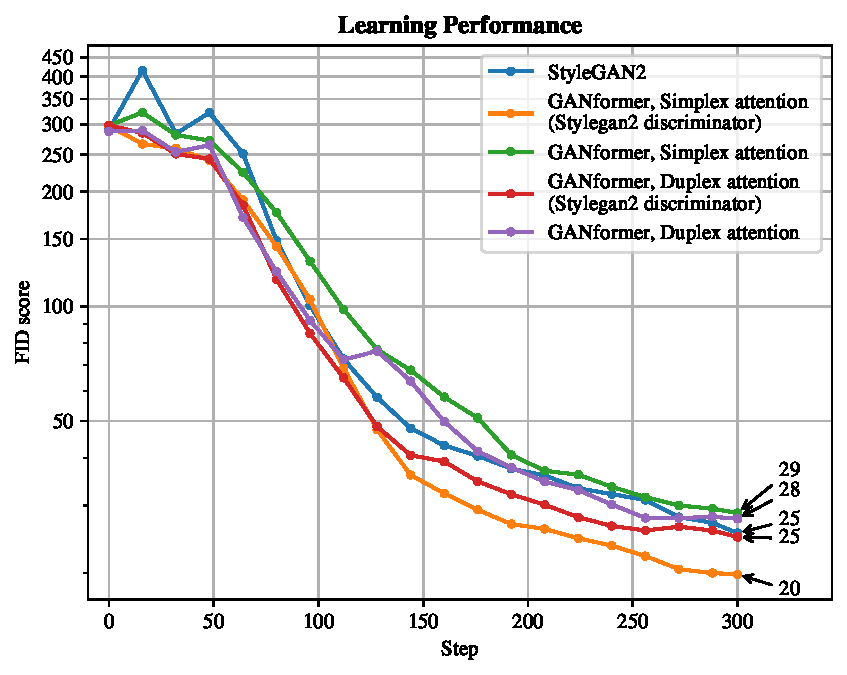
\includegraphics[width=.7\linewidth]{FIDscore-cartoonset.pdf}
	\caption{\textbf{Comparison between the StyleGAN2 and the GANformer models.} We evaluate 
		the models according to FID score along 300k image samples. The score is computed every 
		sixteen checkpoints.}
	\label{fig:performance}
\end{figure*}

As mentioned before, unexpectedly, the model that yields the better results in the original paper, is 
not the best in our experiments.
Not only the FID score is worse than the baseline StyleGAN2 at the final training step, both for 
simplex and duplex attention implementations, but also claims about efficiency cannot be verified.
Models which include attention on the generator only, however, are faster in terms of steps to reach a qualitative results when compared to the baseline.
We believe that this behaviour explains the choices made by the authors in their GitHub publication 
of the code.
Moreover, a comment has to be made on the claim of efficiency: both with and without attention on 
the discriminator, a training step is considerably slower to be completed on the same resources 
when compared to StyleGAN2.
While the latter is capable of having a training speed of 10.9 images generated a second, all flavours 
of the GANformer, in the best case, only yield 8.3 images generated a second.

Finally, to visualise our findings less empirically, we have used random seeds to create latent inputs and shown the resulting images generated by the baseline StyleGAN2 and all four presented variations of the GANformer in Figures \ref{fig:random} and \ref{fig:interpolation} in Appendix \ref{sec:cartoon-results}.

%TODO this is with the old images....
An image generated by each variation is visible in Figure \ref{fig:summaryImgs}.
%\begin{figure}[htb]
%	\centering
%	\includegraphics[width=.9\linewidth]{imgAll_TODO}
%	\caption{\textbf{... using of the various models}.} 
%	\label{fig:summaryImgs}
%\end{figure}
\begin{figure}[htb]
	\centering
	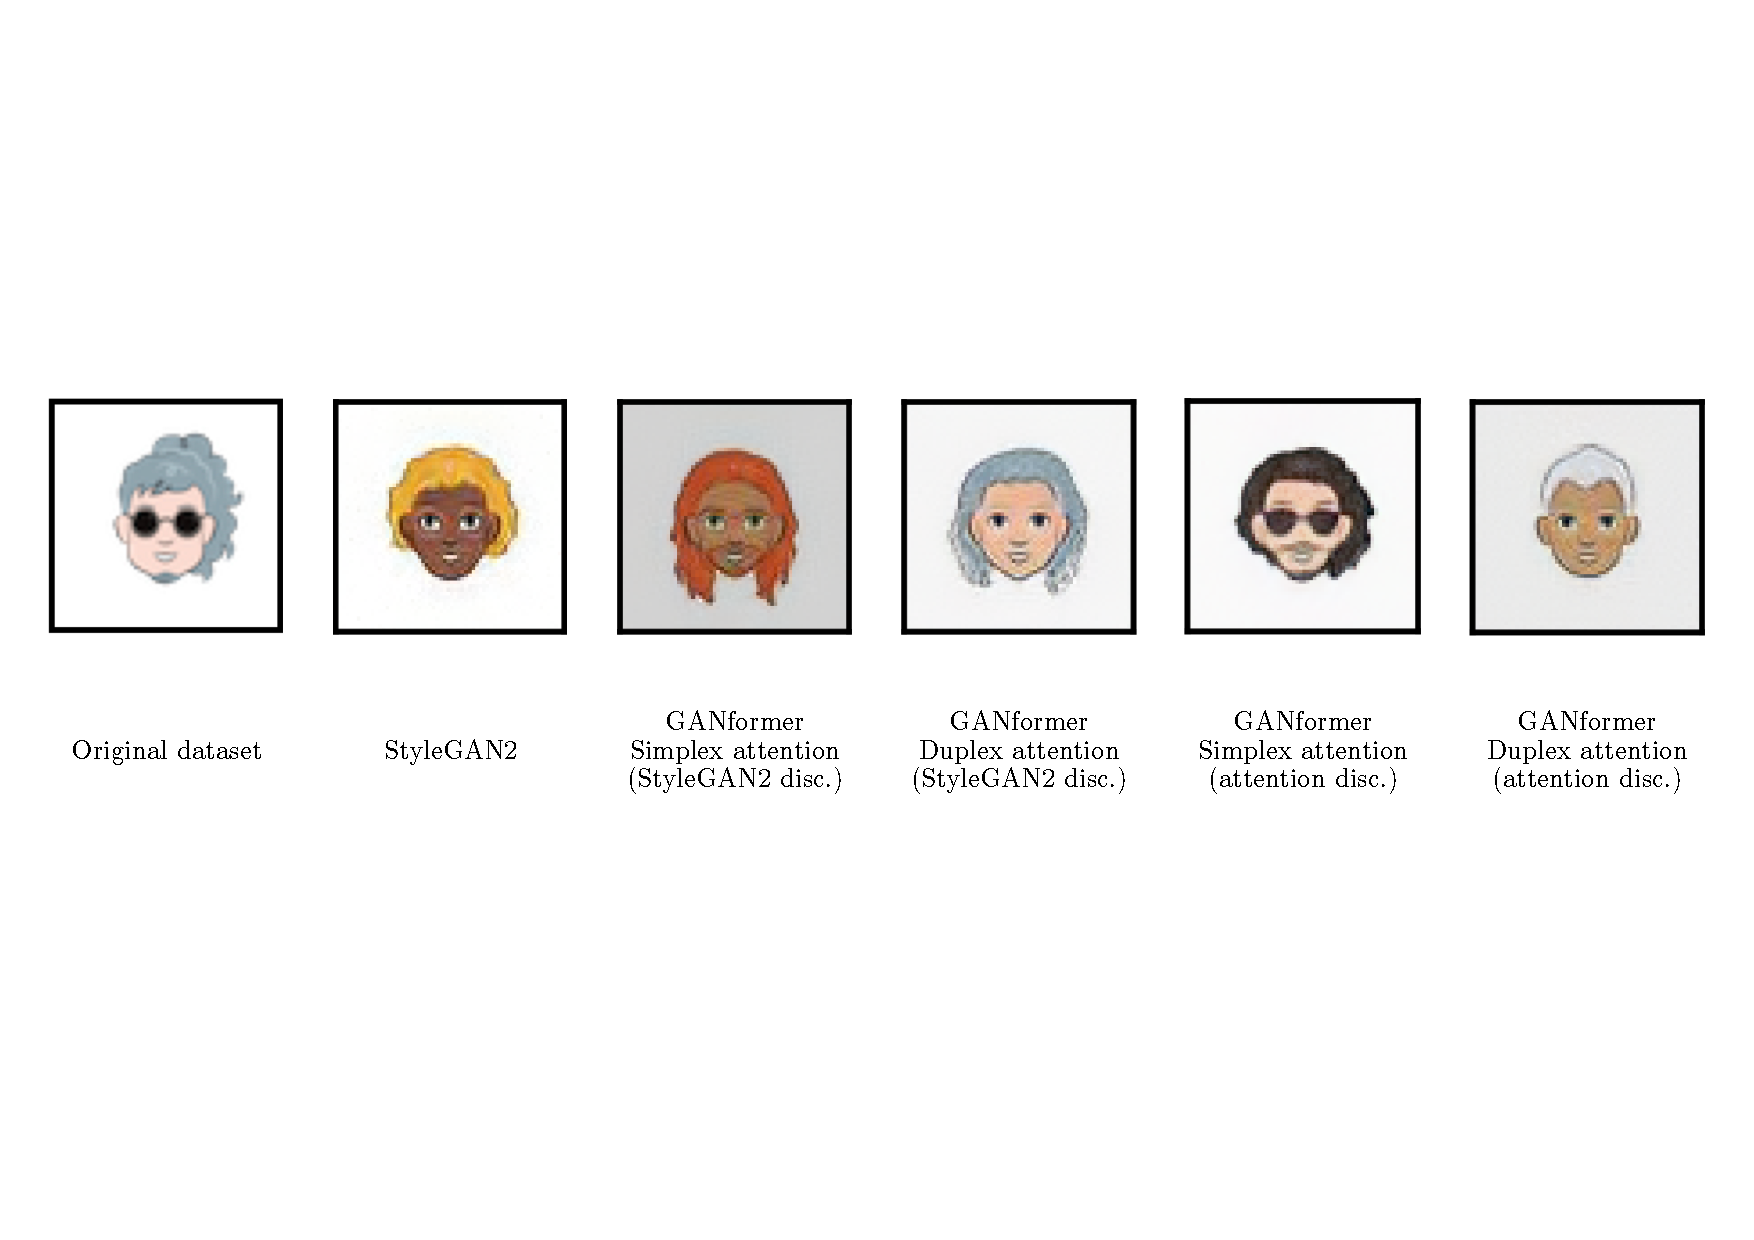
\includegraphics[width=\linewidth]{imgAll}
	\caption{\textbf{... using of the various models}.} 
	\label{fig:summaryImgs}
\end{figure}

\comment{It is blatantly obvious that the Duplex GANformer implementation is not capable of performing the task at hand, while all other models are at least able to produce visually compelling results.
Comparing all outputs to the real images in the original dataset, all except Duplex GANformer tend to create similar results with only background colour differing for models with attention on the generator.}{not true}

\section{FFHQ dataset results}\label{sec:ffhq_results}
For the FFHQ dataset, in Table \ref{tab:results_ffhq} we compared the two GANformer models, both with Duplex attention on the generator, one with attention on the discriminator too and the other with a vanilla StyleGAN2 discriminator.
To have a fair comparison, the three image synthesis methods are run for the same amount of 
iterations.
\begin{table}[htb]
	\centering
	\caption{\textbf{Comparison between the GANformer (Simplex and Duplex) both with and without 
	attention on the Discriminator and competing StyleGAN2}. In the last column, is reported the percentage of improvement all the models, in terms of FID score, with respect to the baseline StyleGAN2 architecture.}
	\label{tab:results_ffhq}
	\vspace{3mm}
	\small
	\begin{tabular}{l|rrrrr}
		\toprule
		\textbf{Model}  & \textbf{FID $\downarrow$}  & \textbf{IS $\uparrow$} & 
		\textbf{Precision$\uparrow$}  & \textbf{Recall $\uparrow$} & \textbf{FID Improvement (\%)}\\ 
		\midrule
		StyleGAN2                    				&  \textbf{40.22} &  &  &  & 0 \%\\ 
		GANformer, Simplex attention & 45.71 & 3.35 &  &  & -13.65 \%\\ 
		GANformer, Duplex attention  & {53.48} & 3.35 & 0.48& 0.0033 & -32.97 \%\\ 
		GANformer, Simplex attention (StyleGAN2 disc.)  &   &   &   &  &  \%\\ 
		GANformer, Duplex attention (StyleGAN2 disc.)  &  {43.66}  & \textbf{3.61} &   \textbf{0.55}   & \textbf{0.0078} & -{8.55} \%\\ 
		\bottomrule
	\end{tabular}
\end{table}

Once again, we can see that the model with multiple attention is considerably worse than the model with attention only in the generator. 

\begin{figure*}[htpb]				
	\centering
%	\raggedleft
	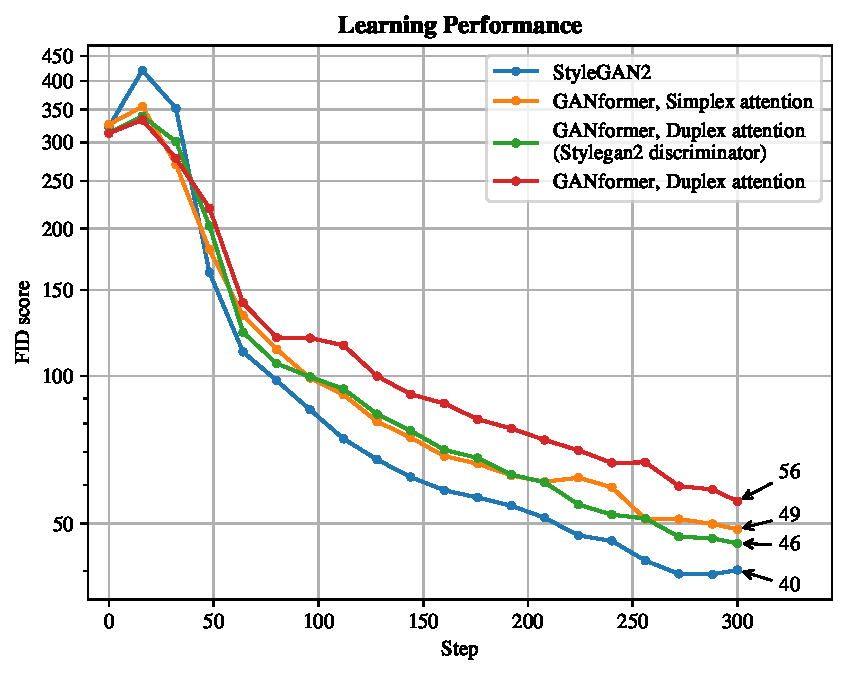
\includegraphics[width=.7\linewidth]{FIDscore-ffhq.pdf}
	\caption{\textbf{Comparison between the StyleGAN2 and the GANformer models.} We evaluate 
	the models according to FID score along 300k image samples. The score is computed every 
	sixteen checkpoints.}
	\label{fig:performance-ffhq}
\end{figure*}

Finally, to visualise our findings less empirically, as for the previous dataset, we have used random seeds to create latent inputs and shown the resulting images generated by the baseline StyleGAN2 and all four presented variations of the GANformer in Figures \ref{fig:random-ffhq} and \ref{fig:interpolation-ffhq} in Appendix \ref{sec:ffhq-results}.

%TODO this is with the old images....
An image generated by each variation is visible in Figure \ref{fig:summaryImgs}.

\begin{figure}[htb]
	\centering
	\includegraphics[width=\linewidth]{ffhq-imgAll}
	\caption{\textbf{... using of the various models}.} 
	\label{fig:summaryImgs-ffhq}
\end{figure}

\section{Discussion and conclusion}
\comment{...}{All this section should be revised since we are using also another dataset}

%	Here you can express your judgments and draw your conclusions based on the  evidences 
%	produced on the previous sections.
%	
%	Try to summarise the achievements of your project and its limits, suggesting (when appropriate) 
%	possible extensions and future works.

In this project we have discussed the replication of ``\emph{Generative adversarial Transformers}'' 
by 
\citet{hudson2021generative}.
Contrary to our initial expectations, in our opinion, some of the claims made by the authors were 
misleading or unproven in a scientific manner.
Once we made this realisation, our methodology shifted from a pure reproduction of the results to a 
search of undisclosed variations of the novel GANformer system in the published material trying to 
obtain 
results that were comparable to the given ones.
As mentioned in Section \ref{sec:comput_req}, our limited resources forced us to reduce the depth 
of our experiments 
compared to the authors'.
We had to shift from four datasets to a single, size-reduced one: \citet{cartoonset}, significantly 
decreasing the time of execution and the complexity of our research.
For the same reasons, we have discarded four out of the five baselines: GAN, k-GAN, SAGAN and 
VQGAN 
in favour of just StyleGAN2.
The choice of StyleGAN2 as the baseline was prompted by a similarity of its execution to the novel 
GANformer, where parts of the author's code are a carbon copy of the StyleGAN2 implementation 
first 
proposed in \citet{karras2019style}.

In this study, we have firstly implemented a Google Colab Pro compatible version of the authors 
code, 
enabling us to train and test StyleGAN2 and the two flavours of GANformer (Duplex and Simplex 
attention) 
in less than 54 hours in total.
As presented in Section \ref{sec:results}, we were not able to achieve the improvements declared by 
the authors but instead 
found a decrease both in time performance and quality.
Believing it was an error arisen by our adaptation we have analysed the pre-trained models provided 
and 
noticed an alarming discrepancy between the code and the methodology discussed in the paper.
In ``\emph{Generative adversarial Transformers}'' by \citet{hudson2021generative}, the attention 
component 
is said to be placed both on the generator and the discriminator sub-networks, while in all the 
pre-trained 
models provided, it seems to never be used on the discriminator.
%Proofreading the code, a BUG has been discovered by us, the optional attention flag, even if set to 
%True 
% when selecting a network structure, is never read during model preparations, resulting in models 
%that never 
% make use of attention in the discriminator phase.
%Moreover, to us it seemed that a discrepancy could be found in the Hyper-parameters settings.


Believing that all of the authors experiments were performed on a different network than the one 
presented 
in the publication, we have tried to recreate the structure that could have yielded the claimed 
qualitative results.
To perform such a task we have decomposed the GANformer network in two sections by keeping 
the presented 
Generator but substituting the hypothetically valid discriminator network with a vanilla StyleGAN 
discriminator.

To our surprise, the StyleGAN/GANformer hybrid performed significantly better than the baseline. In 
the case of duplex attention on the discriminator, we believe that introducing k-means will find the 
centroid/mean of multiple regions of the cartoon face and merge them into one representative region 
of the cartoon face, which will make the discriminator unable to accurately tell the difference 
between a fake image and a real image. Furthermore, the generator tries to maximise the 
discriminator's output for the generated fake image \cite{gulrajani_improved_2017, 
	arjovsky_wasserstein_2017}, which will create shapes that are close to what the discriminator 
	sees 
from the real images confusing the discriminator from differentiating fake and real images.

In conclusion, we have successfully reproduced the ``\emph{Generative Adversarial Transformers}'' 
by \citet{hudson2021generative} and found unexpected results.
We have then modified the proposed methodologies to obtain an image generation network that 
takes inspiration from the 
novel GANformer and adapts it to produce images that score significantly higher than the baseline 
over four quality metrics.

\section{Authors contribution}
\comment{review}{use the standard CRediT authorship contribution statement}
All the authors analysed the original article and the code provided by the creators. 
They took together all the important decisions, either regarding the organisation of the work and the 
problems that have arisen.

Stefano dealt with the dataset preparation and preprocessing phase. He also adapted the StyleGAN2 
baseline for Colab and performed the training loop.

Felix dealt with the given code and take charge of merging the StyleGAN2 and GANformer models, 
adapting the code so that it reproduced carefully what was written in the paper.

Stefano and Giorgia collaborated on the adaptation of the style transformer for StyleGAN2 and later 
on the adaptation of the image visualisation for the GANformer, and in general with the generation 
of images and videos. 

Stefano and Felix worked together on the style mixing adaptation for the GANformer, and since only 
they had available the GPU resources from Google Colab, they also handled with the models training.

Stefano also concentrated on the code refactoring phase, mainly cleaning the code related to the 
discriminator GANformer.

Giorgia focused on the main conceptual ideas behind the original work, and performed a theoretical 
research on the topic and related works. 
Later she drafted this manuscript, with inputs from the other authors which provided critical 
feedback on it. 

All the authors discussed and interpret the results and finally contribute to the final version of this 
article.

\clearpage
\appendix
%	\section{Background and methodology}\label{sec:appendix}
%	
%	\subsection{Background} \label{subsec:app_background}
%	As aforementioned in Section \ref{sec:gan}, GANs \cite{goodfellow2014generative}, are 
%	deep-learning-based generative models composed by two main neural networks: 
%	the \textit{generator} ${G(z)}$, which take as input a sample from the latent space $z$, or a vector 
%	drawn randomly from a Gaussian distribution, and use it to generate new plausible examples in the 
%	problem domain — images in our case — , and the \textit{discriminator} ${D(x)}$, which takes an 
%	example from the domain as input, and predicts a binary class label which classify the examples as 
%	real (coming from the training dataset) or fake (generated by $G$). 
%	
%	The two models are trained together: the discriminator $D$ estimates the probability that 
%	sample $x$ is generated by $G$ or is a real sample, and aims at maximising the probability of 
%	assigning the correct label to both real and fake samples, while the generator $G$ is trained to 
%	maximise the probability of the discriminator $D$ making a mistake, so it aims to minimise 
%	$\log(1-D(G(z))))$.
%	
%	Combining the two objectives for $G(z)$ and $D(x)$ we get the \textit{GAN min-max game} with the 
%	value function $V(G,D)$:
%	\begin{equation}
%		\label{e:minmaxgame}
%		\min_G \max_D V(G,D) = 
%		\mathbb{E}_{x \sim p*(x)} [\log D(x)] + \mathbb E _{z \sim p_z(z)} [\log (1-D(G(z))))]
%	\end{equation}
%	
%	GANs typically work with images, as in our case, for this reason, both the generator and 
%	discriminator models use Convolutional Neural Networks (CNNs).
%	\begin{figure*}[htb]				
%		\centering
%		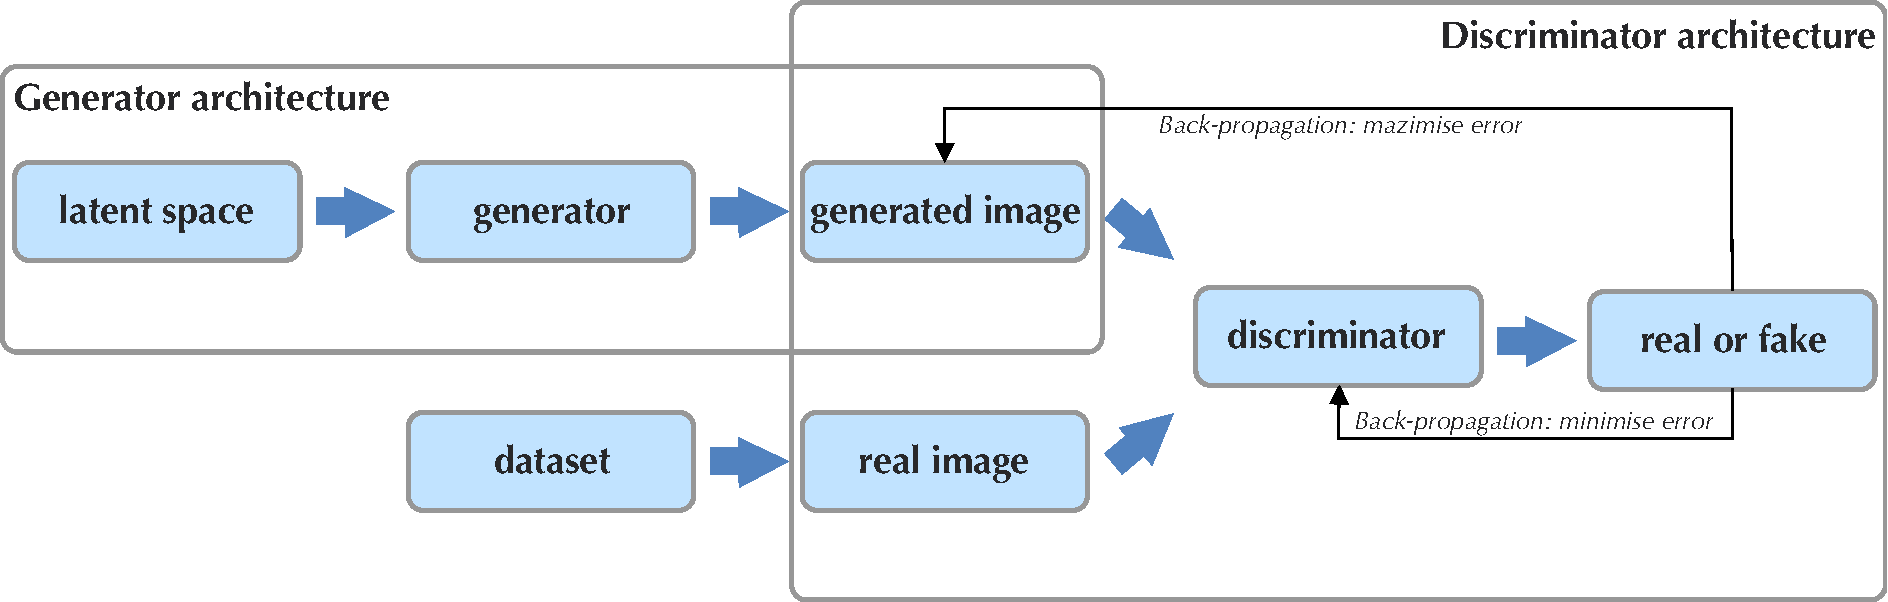
\includegraphics[width=.65\linewidth]{images/GAN}
%		\caption{\textbf{GAN architecture.} Visualisation of the two components of a GAN: generator and 
%			discriminator.}
%		\label{fig:gan}
%	\end{figure*}
%	
%	In this paper, we exploited StyleGAN2 architecture, the second version of the StyleGAN model, 
%	introduced in Section \ref{sec:StyleGAN}, which is a re-design of the GANs generator architecture.
%	The aim of the StyleGAN is to control the image synthesis process \cite{karras2019style}. The 
%	architecture is illustrated in Figure \ref{fig:StyleGAN}.
%	\begin{figure*}[!h]				
%		\centering
%		\includegraphics[width=.5\linewidth]{images/StyleGAN}
%		\caption{\textbf{StyleGAN architecture.} Re-design of the traditional GAN generator into a 
%			style-based generator.}
%		\label{fig:StyleGAN}
%	\end{figure*}
%	
%	The StyleGAN approach departs from the design of a common generator network, consisting in a 
%	multi-layer CNN.
%	A traditional GAN generator feeds the latent code $z$ though the input layer only, to start the 
%	up-sampling process.
%	\citet{karras2019style} introduce a feed-forward mapping network $f : Z \rightarrow W$ which 
%	processes the latent code $z$ in the input latent space $Z$, and output an intermediate latent 
%	vector $w \in W$. 
%	$w$, in turn, interacts directly with each convolution through the synthesis network  $g$ and, in 
%	particular, with the \textit{Adaptive Instance Normalisation (AdaIN)} \cite{huang2017arbitrary} aligns 
%	the mean and variance of the content features with those of the style features, meaning that is able 
%	to globally controls these parameters and so the strength of image features at different scales. 
%	
%	The \textit{AdaIN} operation is defined as:
%	\begin{equation}
%		\label{e:adain}
%		\mathsf{AdaIN}(x, y) = \sigma(y) \bigg(\frac{x - \mu(x)}{\sigma (x)} \bigg) + \mu (y) \mbox{,}
%	\end{equation}
%	where $x$ is the content input, $y$ a style input, and the channel-wise mean and variance of $x$ 
%	are aligned to match those of $y$.
%	
%	\citet{karras2019style} provided the generator with a direct means to generate stochastic 
%	details by 
%	introducing explicit Gaussian noise inputs after each convolution: an automatic and 
%	unsupervised 
%	separation of high-level attributes (e.g., pose, identity) from stochastic variation (e.g., 
%	freckles, hair) 
%	is obtained in the generated images, and intuitive scale-specific mixing and interpolation 
%	operations 
%	are enabled.
%	
%	StyleGAN2 \cite{karras2020analyzing} are a revisiting of the architecture of the StyleGAN synthesis 
%	network. Figure \ref{fig:StyleGAN2} shows the various changes made to the original architecture up 
%	to the final network.
%	\begin{figure*}[htb]				
%		\centering
%		\includegraphics[width=.9\linewidth]{images/StyleGAN2}
%		\caption{\textbf{StyleGAN2 architecture.} Evolution from a StyleGAN to a StyleGAN2 synthesis 
%			network.}
%		\label{fig:StyleGAN2}
%	\end{figure*}
%	
%	In particular, some redundant operations have been removed from the original StyleGAN architecture.
%	Bias and noise are operations which might have conflicting interests, and their application within the 
%	style block caused their relative impact to be inversely proportional to the current style’s 
%	magnitudes. For this reason, they have been moved outside the style block and separated, allowing 
%	to obtain more predictable results.
%	Furthermore, after this change, the mean is no longer necessary, but it is sufficient for the 
%	normalisation and modulation to operate on the standard deviation alone.
%	Moreover, the application of bias, noise, and normalisation to the constant input has been safely 
%	removed. 
%	
%	When the style block consists in a modulation, a convolution, and a normalisation operation, it is 
%	possible to restructure the AdaIN has a demodulation operation, which is applied to the weights 
%	associated with each convolution layer. 
%	AdaIN uses different scale and shift parameters to align different areas of $w$ — the activations 
%	of intermediate activations — with different regions of the feature map (either within each feature 
%	map or via grouping features channel-wise by spatial location), while weight demodulation takes the 
%	scale and shift parameters out of a sequential computation path, instead baking scaling into the 
%	parameters of convolutional layers.
%	
%	%	The \textit{mapping network}, which consists in a series of feed-forward layers, whose 
%	%	objective is to convert the sampled latents from a normal distribution $z$ to the intermediate 
%	%	space $w$. The $k$ latent components either are mapped independently or interact with each 
%	%	other through self-attention.
%	%	The \textit{synthesis network} is composed by multiple layers of convolution where the 
%	%	images features begin from a small constant/sampled grid and up-sampling until reaching the 
%	%	desirable resolution.
%	%	After each convolution, the image features are modulated by the intermediate latent vectors 
%	%$w$, 
%	%	meaning that their variance and bias are controlled. 
%	
%	Also transformers are an important deep-learning model exploited in this work and introduced in 
%	Section \ref{sec:transformer}. 	
%	An \textit{attention function} \cite{vaswani2017attention}, can be described as mapping a query and 
%	a set of key-value pairs to an output, where the query, keys, values, and output are all vectors. The 
%	output is computed as a weighted sum of the values, where the weight assigned to each value is 
%	computed by a compatibility function of the query with the corresponding key.
%	
%	The input consists of queries and keys of dimension $d_k$, and values of dimension $d_v$. The dot 
%	products of the query with all keys is computed, each divided by $\sqrt{d_k}$ and then a 
%	softmax function is applied to obtain the weights on the values.
%	In practice, the attention function is computed on a set of queries simultaneously, packed together 
%	into a matrix $Q$. The keys and values are also packed together into matrices $K$ and $V$. 
%	\begin{equation}
%		\label{eqn:attention}
%		\mathsf{Attention}(Q, K, V) = \mathsf{softmax} \big( \frac{QK^T}{\sqrt{d_k}}\big)V
%	\end{equation}
%	% This is a \textit{dot-product attention} with a scaling factor of $\sqrt{1}$. 
%	Instead of performing a single attention function, transformers use multiple self-attentions, called 
%	\textit{multi-head attention}, allowing the model to jointly attend to information from different 
%	representation subspaces at different positions, learning attention relationship independently	
%	\cite{vaswani2017attention}.
%	As mentioned in	Section \ref{sec:transformer}, \citet{vaswani2017attention} used multiple 
%	multi-head 
%	attentions, which are defined as follows.
%	\begin{equation}
%		\label{eqn:multihead}
%		{\mathsf{MultiHead}(Q, K, V) = \mathsf{Concat}(\mathsf{head}_1 \dots, 
%			\mathsf{head}_h) W^O }
%		\mbox{,}
%	\end{equation}
%	where $ \mathsf{head}_i = \mathsf{Attention}(QW_i^Q, KW_i^K , VW_i^V)$, and the 
%	projections are parameter matrices $W_i^Q \in \mathbb{R}^{d_{\text{model}}\times 
%		d_k}$, $W_i^K \in \mathbb{R}^{d_{\text{model}}\times d_k}$, $W_i^V \in 
%	\mathbb{R}^{d_{\text{model}}\times d_v}$ and $W^O \in \mathbb{R}^{hd_v \times 
%		d_{\text{model}}}$.
%	
%	As reported by \cite{vaswani2017attention}, transformer uses multi-head attention in three 
%	different 
%	ways:
%	\begin{enumerate}
%		\item In "encoder-decoder attention" layers, the queries come from the previous decoder 
%		layer, 
%		and the memory keys and values come from the output of the encoder. This allows every 
%		position in the decoder to attend over all positions in the input sequence.
%		\item The encoder contains self-attention layers, in which all of the keys, values 
%		and queries come from the output of the previous layer in the encoder. 
%		Each position in the encoder can attend to all positions in the previous layer of the encoder.
%		\item Similarly, self-attention layers in the decoder allow each position in the decoder to 
%		attend 
%		to all positions in the decoder up to and including that position. We need to prevent leftward 
%		information flow in the decoder to preserve the auto-regressive property. We implement 
%		this 
%		inside of scaled dot-product attention by masking out (setting to $-\infty$) all values in the 
%		input of the softmax which correspond to illegal connections. 
%	\end{enumerate}
%	
%	%	At each step the model is auto-regressive, consuming the previously generated symbols as 
%	%	additional input when generating the next.
%	%		\begin{enumerate*}
%	%			\item[(1)] a \textit{multi-head self-attention mechanism} working in parallel, and 
%	%			\item[(2)] a \textit{position-wise fully connected feed-forward neural network}, with 
%	%residual 
%	%			connections followed by normalisation.
%	%	\end{enumerate*}
%	%	Moreover, the decoder self-attention sub-layer has a mask which prevents positions from 
%	%	attending 
%	%	to subsequent positions (so positional encoding provided as additional input to bottom 
%	%layer). 
%	%	This, combined with fact that the output embeddings are offset by one position, ensures 
%	%that 
%	%	the predictions for position $i$ can depend only on the known outputs at positions less 
%	%than $i$.
%	% 	In addition, the decoder has a third sub-layer, which performs \textit{multi-head attention} 
%	%over 
%	%	the output of the encoder stack. 
%	
%	\subsection{Generative Adversarial Transformers in depth} \label{subsec:app_methodology}
%	In this Section we dive into the details of Generative Adversarial Transformers 
%	\cite{hudson2021generative}, introduced in Section \ref{sec:ganformer}. 
%	
%	The BERT \textit{transformer network} \cite{devlin2019bert} interleaves \textit{multi-head 
%		self-attention} and \textit{feed-forward layers}. Each pair of self-attention and feed-forward 
%	layers is 
%	intended as a \textit{transformer layer}, hence, a transformer is a stack of several such layers. 
%	
%	The \textit{self-attention layer} considers all pairwise relations among the input elements, so to 
%	update each single element by attending to all the others. 
%	The \textit{bipartite transformer} generalises this formulation, featuring instead a bipartite graph 
%	between two groups of variables — in the GAN case, latents and image features. 
%	
%	In particular, the attention layers are added in between the convolutional layers of both the 
%	generator and discriminator.
%	
%	Instead of controlling the style of all features globally, the new attention layer is used to perform 
%	\textit{adaptive region-wise modulation}. The latent vector $z$ is split into $k$ components, 
%	$z = [z_1 , \dots, z_k ]$ and, as in StyleGAN \cite{karras2019style}, pass each of them through a 
%	shared mapping network, obtaining a corresponding set of intermediate latent variables $Y = [y_1 , 
%	...,y_k ]$. 
%	
%	During synthesis, after each CNN layer in the generator, the feature map $X$ and latents $Y$ play 
%	the roles of the two element groups, mediating their interaction through our new attention layer 
%	(either simplex or duplex). 
%	This setting thus allows for a flexible and dynamic style modulation at the region level. 
%	
%	Since soft attention tends to group elements based on their proximity and content similarity, the 
%	transformer architecture naturally fits into the generative task and proves useful in the visual 
%	domain, allowing the model to exercise finer control in modulating local semantic regions. This 
%	capability turns to be especially useful in modelling highly-structured scenes.
%	
%	For the discriminator, attention is applied after every convolution using trained embeddings to 
%	initialise the aggregator variables $Y$, which may intuitively represent background knowledge the 
%	model learns about the task. At the last layer are concatenated these variables $Y$ to the final 
%	feature map $X$ to make a prediction about the identity of the image source. 
%	This structure empowers the discriminator with the capacity to likewise model long-range 
%	dependencies, which can aid it in its assessment of the image fidelity, allowing to acquire a more 
%	holistic understanding of the visual modality.
%	%	\textcolor{blue}{
%	%	\begin{itemize}
%	%		\item Compositional Latent Space with multiple variables that coordinate through 
%	%attention to 
%	%		produce the image cooperatively, in a manner that matches the inherent 
%	%compositionality of 
%	%		natural scenes.
%	%		\item Bipartite Structure that balances between expressiveness and efficiency, 
%	%modelling 
%	%		long-range dependencies while maintaining linear computational costs.
%	%		\item Bidirectional Interaction between the latents and the visual features, which allows 
%	%the 
%	%		refinement and interpretation of each in light of the other.
%	%		\item Multiplicative Integration rule to impact the features' visual style more flexibly, 
%	%akin to 
%	%		StyleGAN but in contrast to the transformer network.
%	%	\end{itemize}
%	%}

\section{Google Cartoon Set results} \label{sec:cartoon-results}
The dataset used in this work is the Google Cartoon Set \cite{cartoonset} introduced in Section 
\ref{sec:dataset}, containing 10k 2D cartoon avatar. These images are composed of 16 components 
that vary in 10 artwork attributes, 4 colour attributes, and 4 proportion attributes (see Table 
\ref{tab:dataset}). 

\begin{table}[htb]
	\centering
	\caption{Attributes of the Cartoon Set.}
	\label{tab:dataset}
	\vspace{3mm}
	\small
	\begin{tabularx}{\textwidth}{ll|r|X}
		&& \textbf{\# Variants} & \textbf{Description}                              \\
		\toprule
		\multirow{10}*{\textbf{Artwork}} 	&	\texttt{chin\_length}           & 3           & Length of 
		chin 
		(below 	mouth region)      \\
		&	\texttt{eye\_angle}             & 3           & Tilt of the eye inwards or outwards      \\
		&	\texttt{eye\_lashes}            & 2           & Whether or not eyelashes are visible     \\
		&	\texttt{eye\_lid}               & 2           & Appearance of the eyelids      	\\
		&	\texttt{eyebrow\_shape}        & 14          & Shape of eyebrows        \\
		&	\texttt{eyebrow\_weight}        & 2           & Line weight of eyebrows           \\
		&	\texttt{face\_shape}            & 7           & Overall shape of the face                \\
		&	\texttt{facial\_hair}           & 15          & Type of facial hair (type 14 is no hair) \\
		&	\texttt{glasses}                & 12          & Type of glasses (type 11 is no glasses)  \\
		&	\texttt{hair}                   & 111         & Type of head hair                        \\
		\midrule
		\multirow{4}*{\textbf{Colors}} &	\texttt{eye\_color}    & 5 & Color of the eye 
		irises           \\
		&	\texttt{face\_color}            & 11          & Color of the face skin                   \\
		&	\texttt{glasses\_color}         & 7           & Color of the glasses, if present         \\
		&	\texttt{hair\_color}        & 10     & Color of the hair, facial hair, and eyebrows      \\
		\midrule
		\multirow{4}*{\textbf{Proportions}} &	\texttt{eye\_eyebrow\_distance} & 3           & 
		Distance 
		between the eye and eyebrows    \\
		&	\texttt{eye\_slant}             & 3           & Similar to eye\_angle, but rotates the eye and 
		does 
		not change artwork  \\
		&	\texttt{eyebrow\_thickness}     & 4           & Vertical scaling of the eyebrows         \\
		&	\texttt{eyebrow\_width}         & 3           & Horizontal scaling of the eyebrows            \\
		\bottomrule                         
	\end{tabularx}
\end{table}

\begin{figure}[htpb]
	\centering
	\begin{subfigure}{\linewidth}
		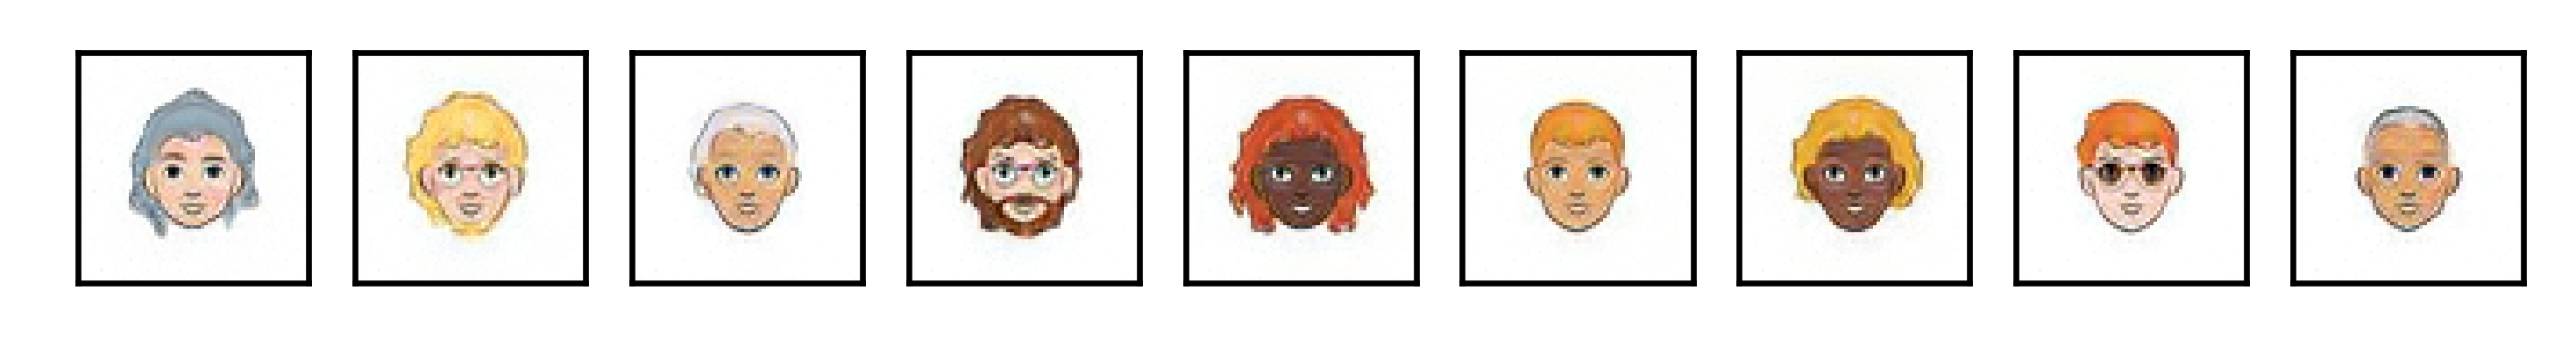
\includegraphics[width=\linewidth]{random_Stylegan2_300kimg.png}
		\vspace{-7mm}
		\caption{StyleGAN2.} 
	\end{subfigure}
	\begin{subfigure}{\linewidth}
		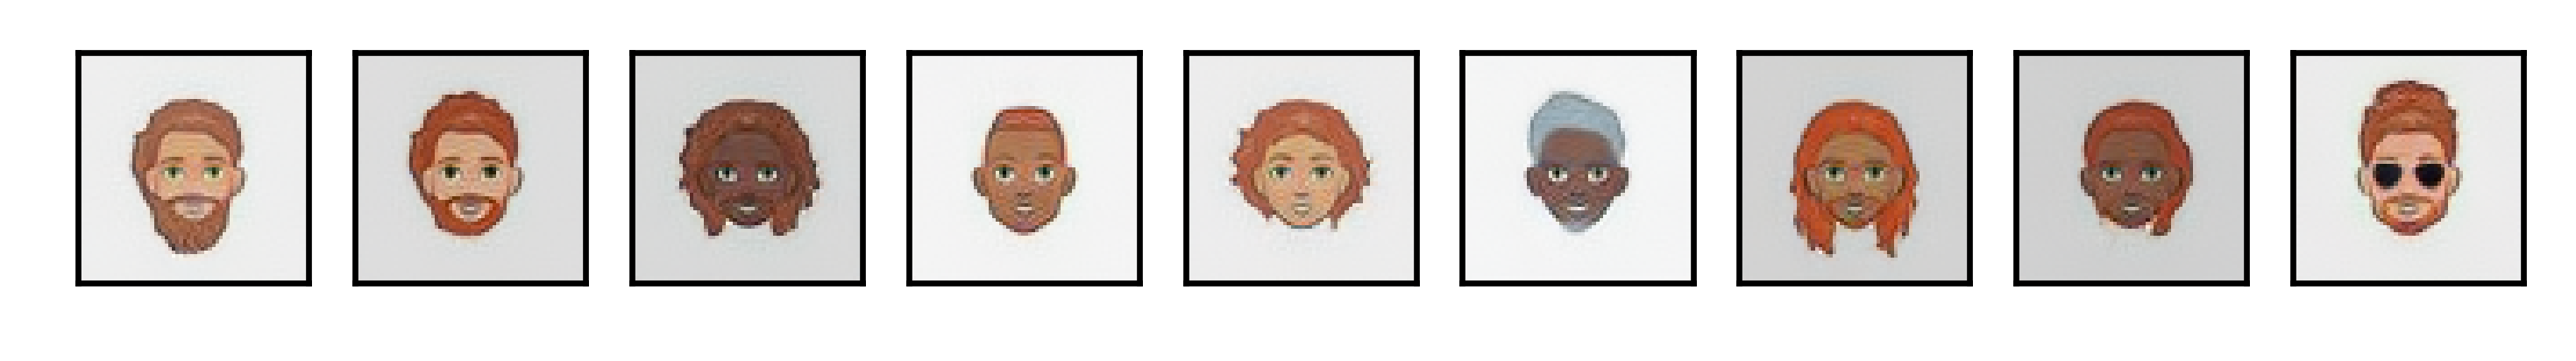
\includegraphics[width=\linewidth]{random_GANFormer_Simplex_D_Stylegan2_300kimg.png}
		\vspace{-7mm}
		\caption{GANformer with Simplex attention and vanilla StyleGAN2 discriminator.}
	\end{subfigure}
	\begin{subfigure}{\linewidth}
		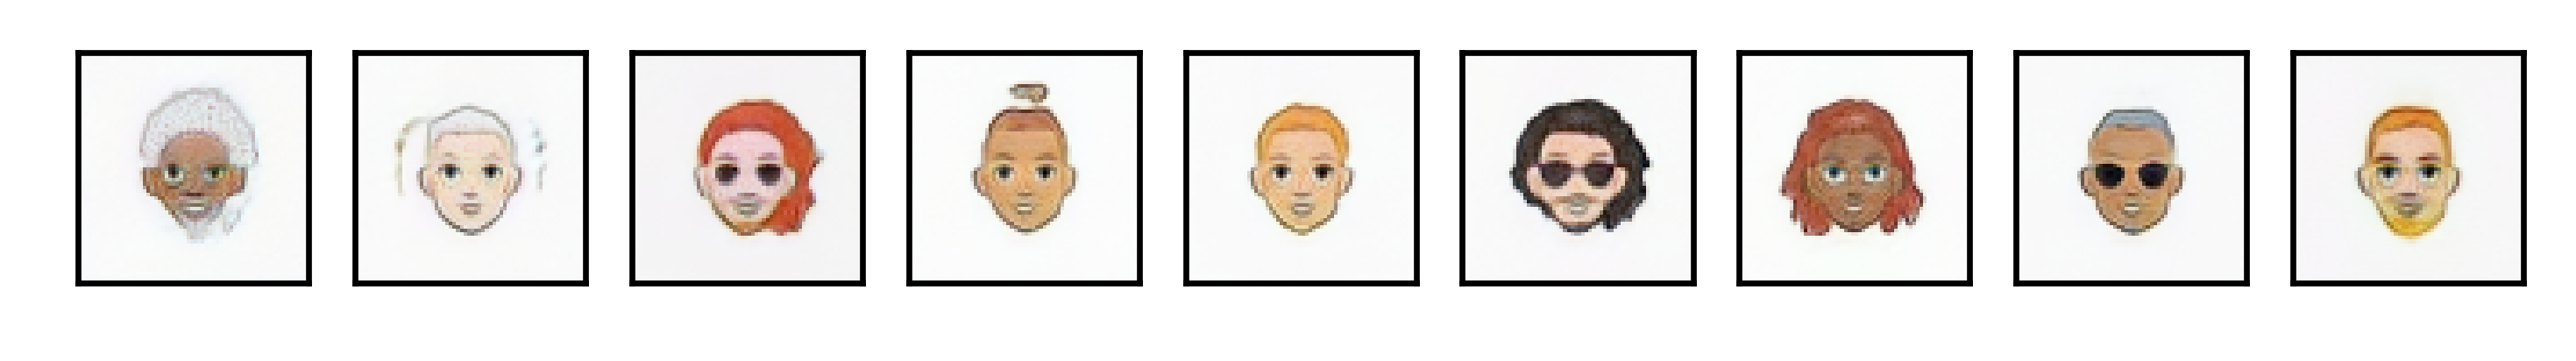
\includegraphics[width=\linewidth]{random_GANFormer_Simplex_D_Att_300kimg.png}
		\vspace{-7mm}
		\caption{GANformer with Simplex attention.}
	\end{subfigure}
	\begin{subfigure}{\linewidth}
		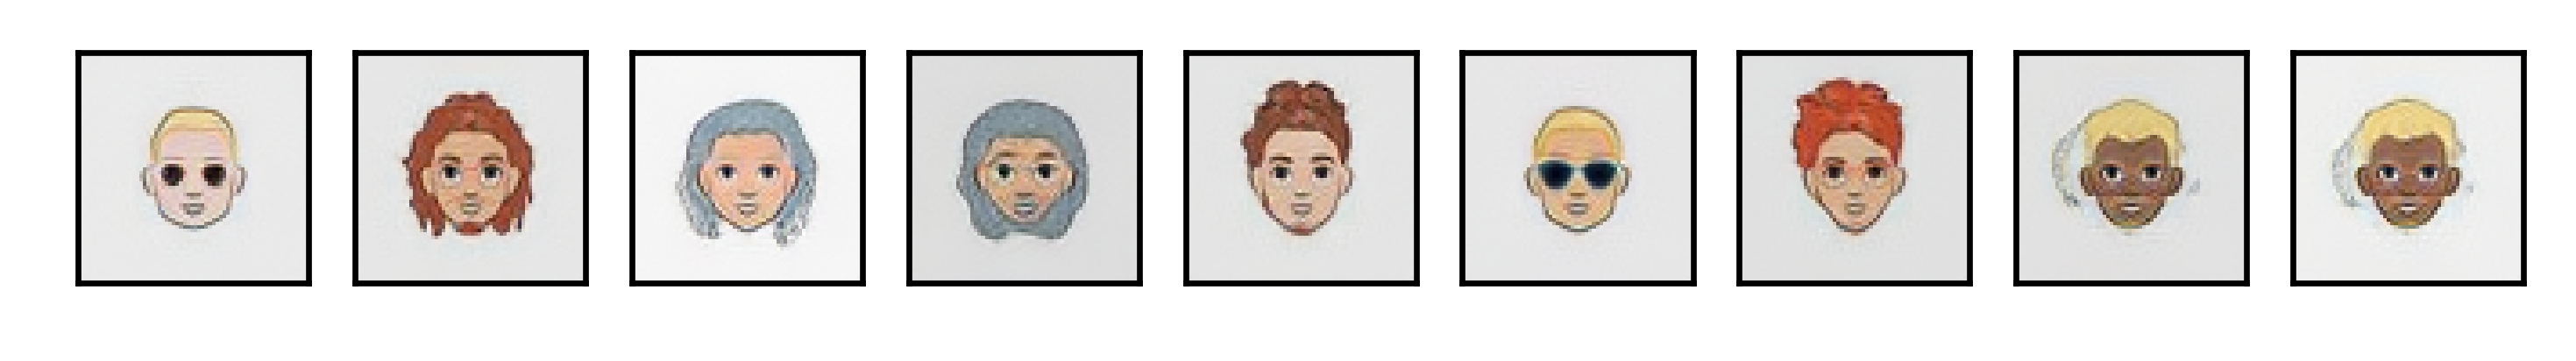
\includegraphics[width=\linewidth]{random_GANFormer_Duplex_D_Stylegan2_300kimg.png}
		\vspace{-7mm}
		\caption{GANformer with Duplex attention and vanilla StyleGAN2 discriminator.}
	\end{subfigure}
	\begin{subfigure}{\linewidth}
		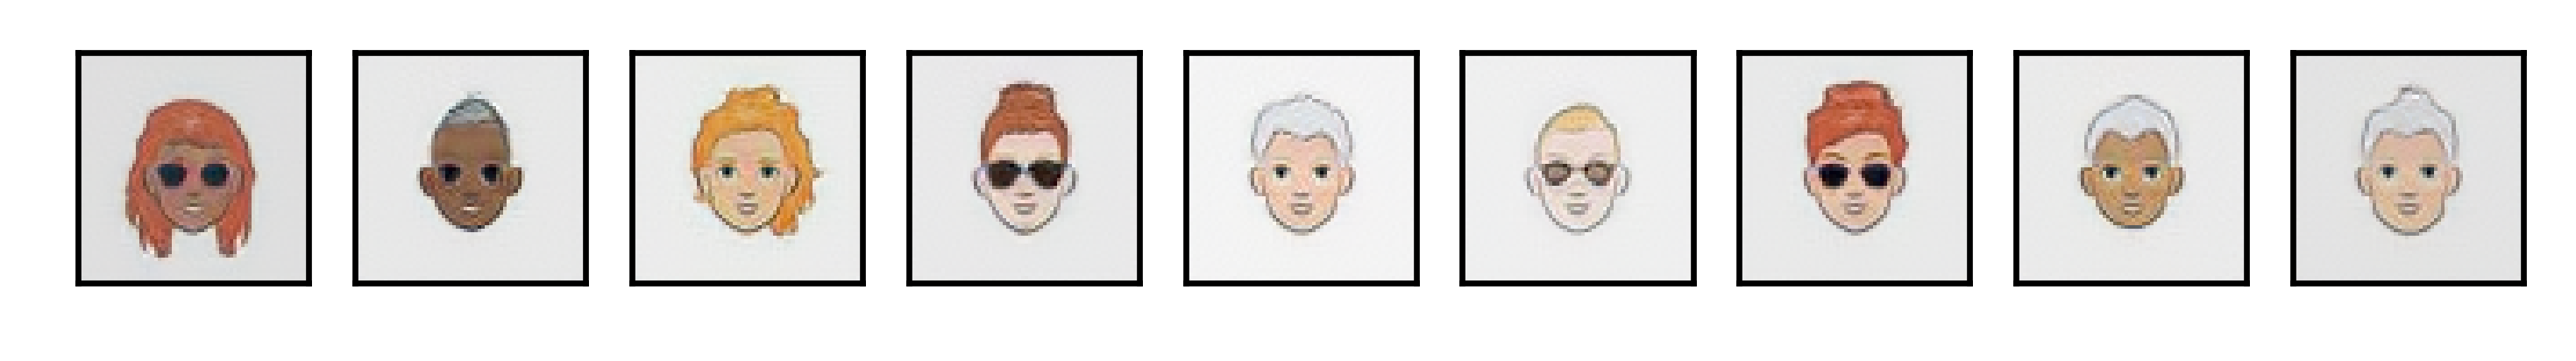
\includegraphics[width=\linewidth]{random_GANFormer_Duplex_D_Att_300kimg.png}
		\vspace{-7mm}
		\caption{GANformer with Duplex attention.}
	\end{subfigure}
	\vspace{3mm}
	\caption{\textbf{Visualisation of 9 images generated with the various models}.}\label{fig:random}
\end{figure}

\begin{figure}[htpb]
	\centering
	\begin{subfigure}{\linewidth}
		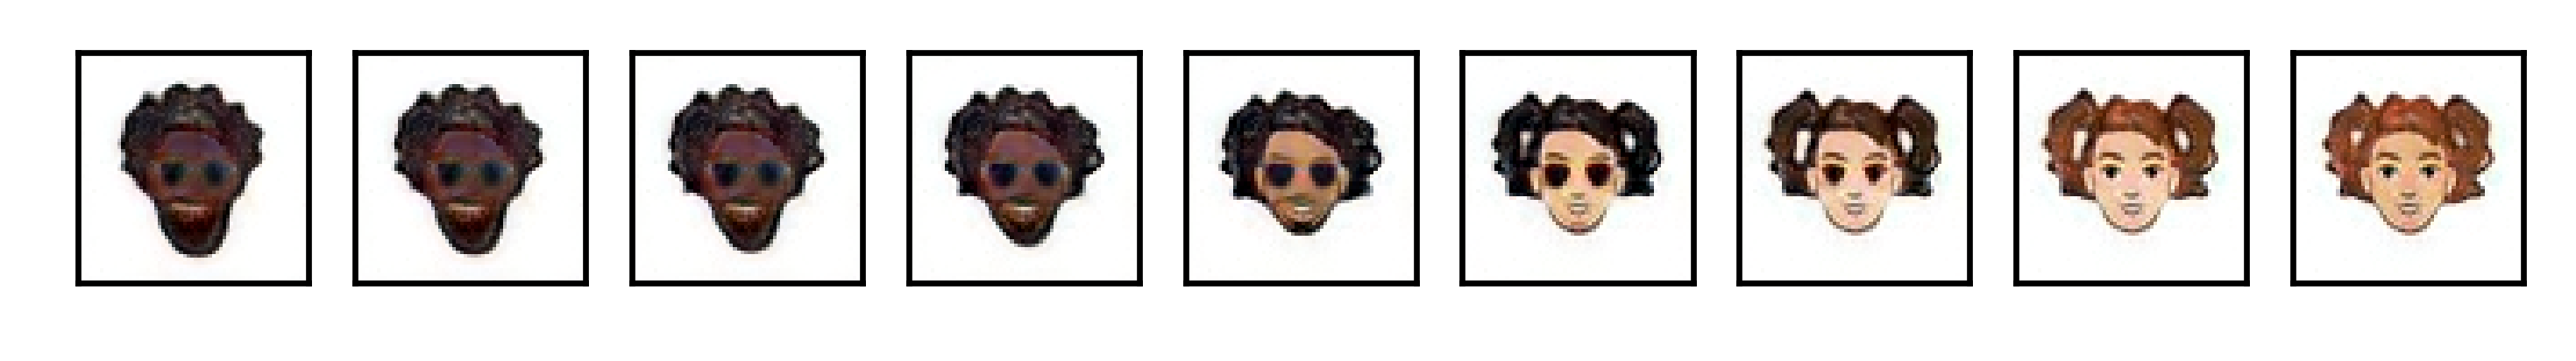
\includegraphics[width=\linewidth]{interpolation_Stylegan2_300kimg.png}
		\vspace{-7mm}
		\caption{StyleGAN2.} 
	\end{subfigure}
	\begin{subfigure}{\linewidth}
		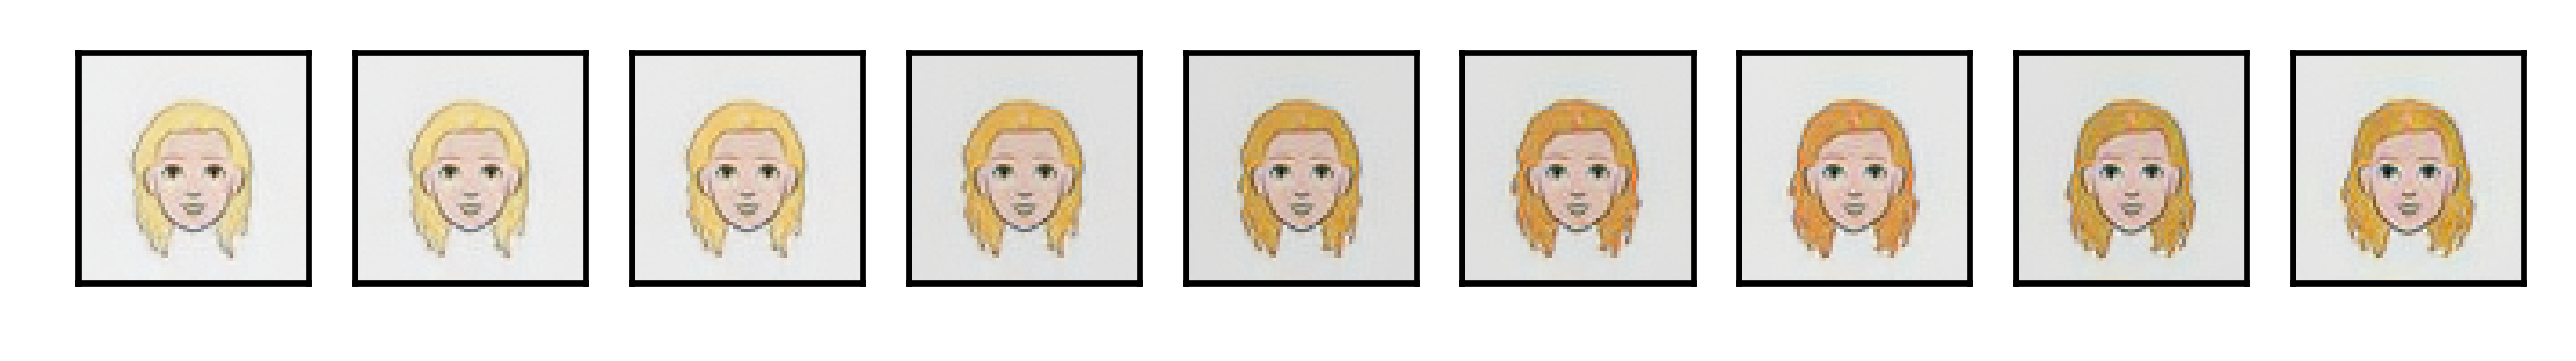
\includegraphics[width=\linewidth]{interpolation_GANFormer_Simplex_D_Stylegan2_300kimg.png}
		\vspace{-7mm}
		\caption{GANformer with Simplex attention and vanilla StyleGAN2 discriminator.}
	\end{subfigure}
	\begin{subfigure}{\linewidth}
		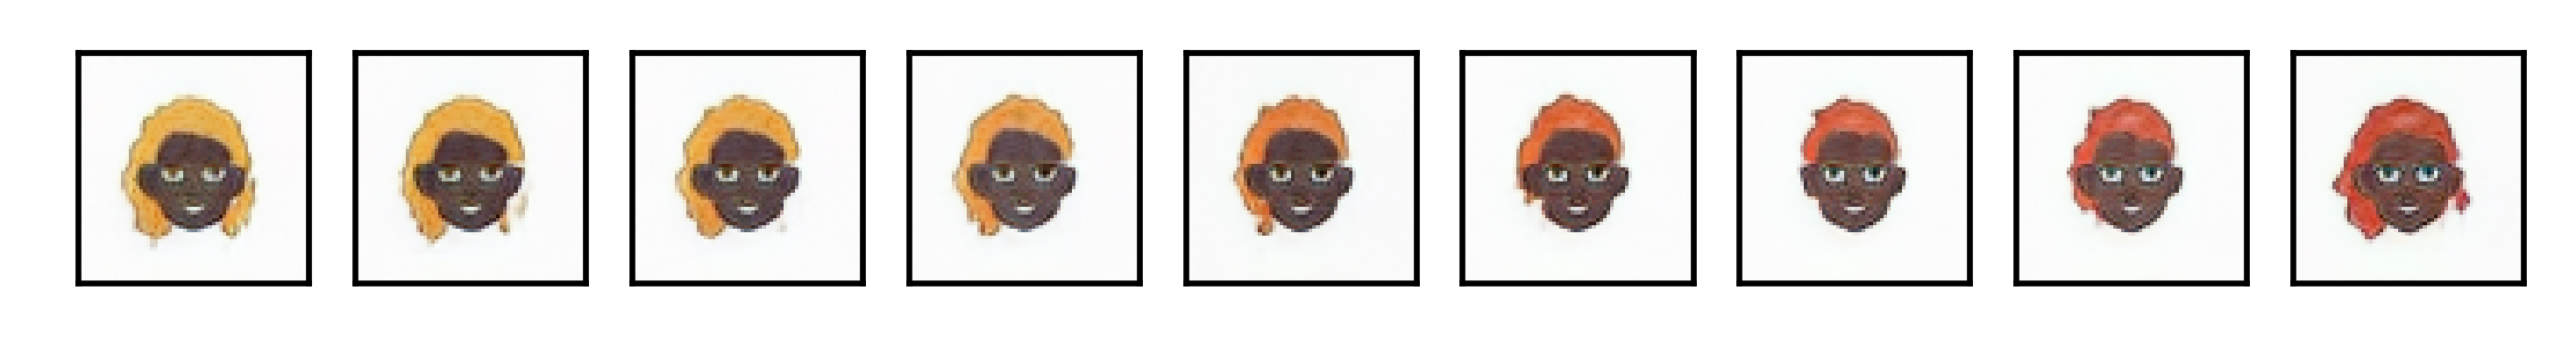
\includegraphics[width=\linewidth]{interpolation_GANFormer_Simplex_D_Att_300kimg.png}
		\vspace{-7mm}
		\caption{GANformer with Simplex attention.}
	\end{subfigure}
	\begin{subfigure}{\linewidth}
		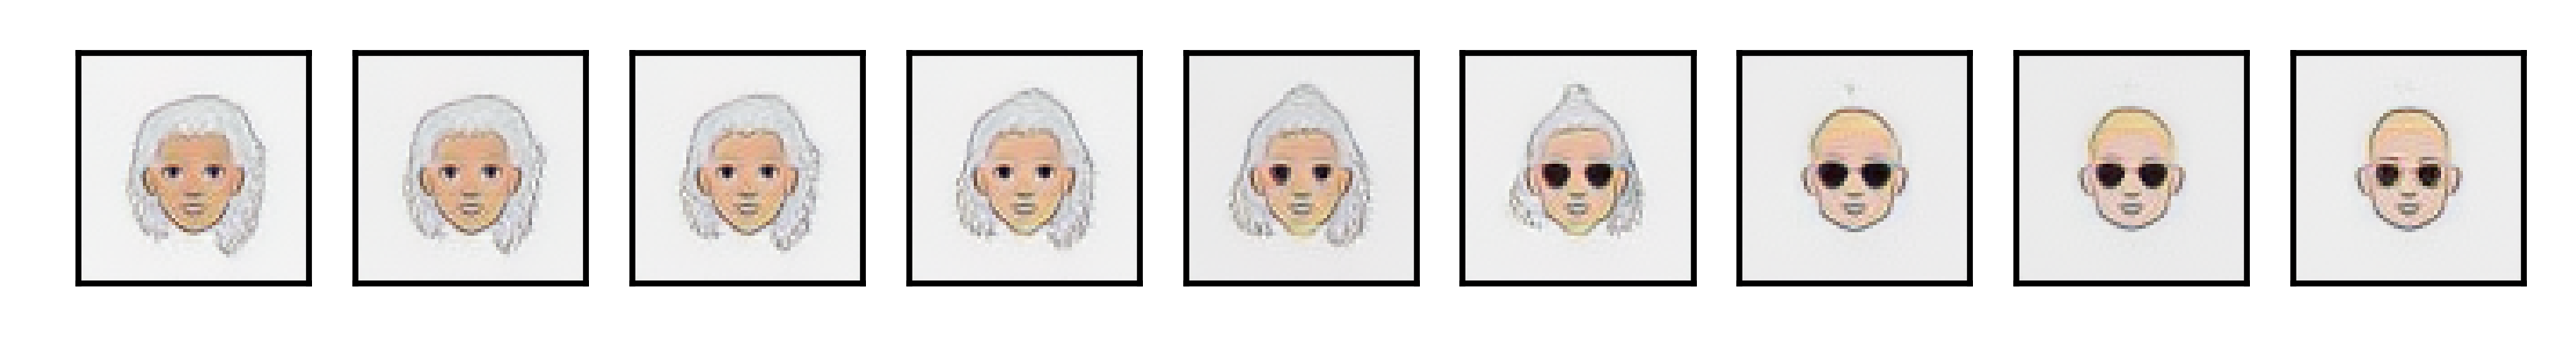
\includegraphics[width=\linewidth]{interpolation_GANFormer_Duplex_D_Stylegan2_300kimg.png}
		\vspace{-7mm}
		\caption{GANformer with Duplex attention and vanilla StyleGAN2 discriminator.}
	\end{subfigure}
	\begin{subfigure}{\linewidth}
		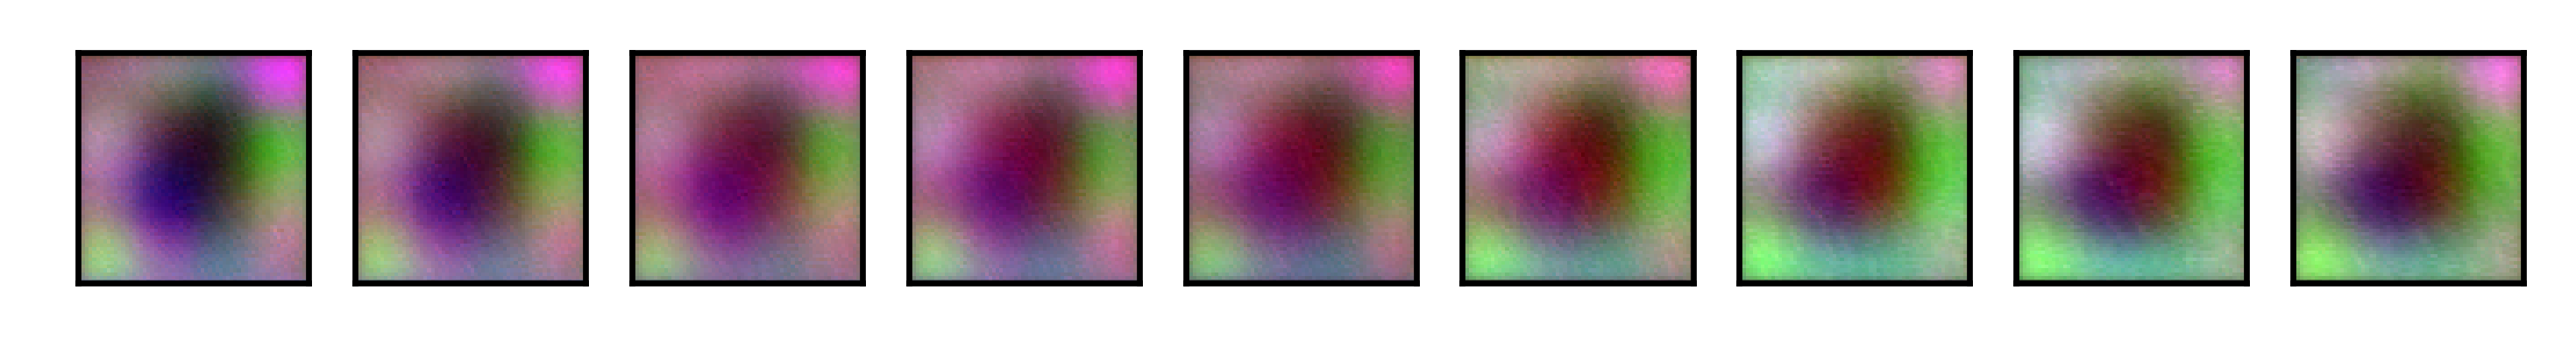
\includegraphics[width=\linewidth]{interpolation_GANFormer_Duplex_D_Att_300kimg.png}
		\vspace{-7mm}
		\caption{GANformer with Duplex attention.}
	\end{subfigure}
	\vspace{3mm}
	\caption{\textbf{Simple $\mathbf{z}$ interpolation using of the various models}.} 
	\label{fig:interpolation}
\end{figure}



\section{FFHQ dataset results} \label{sec:ffhq-results}
\begin{figure}[htpb]
	\centering
	\begin{subfigure}{\linewidth}
		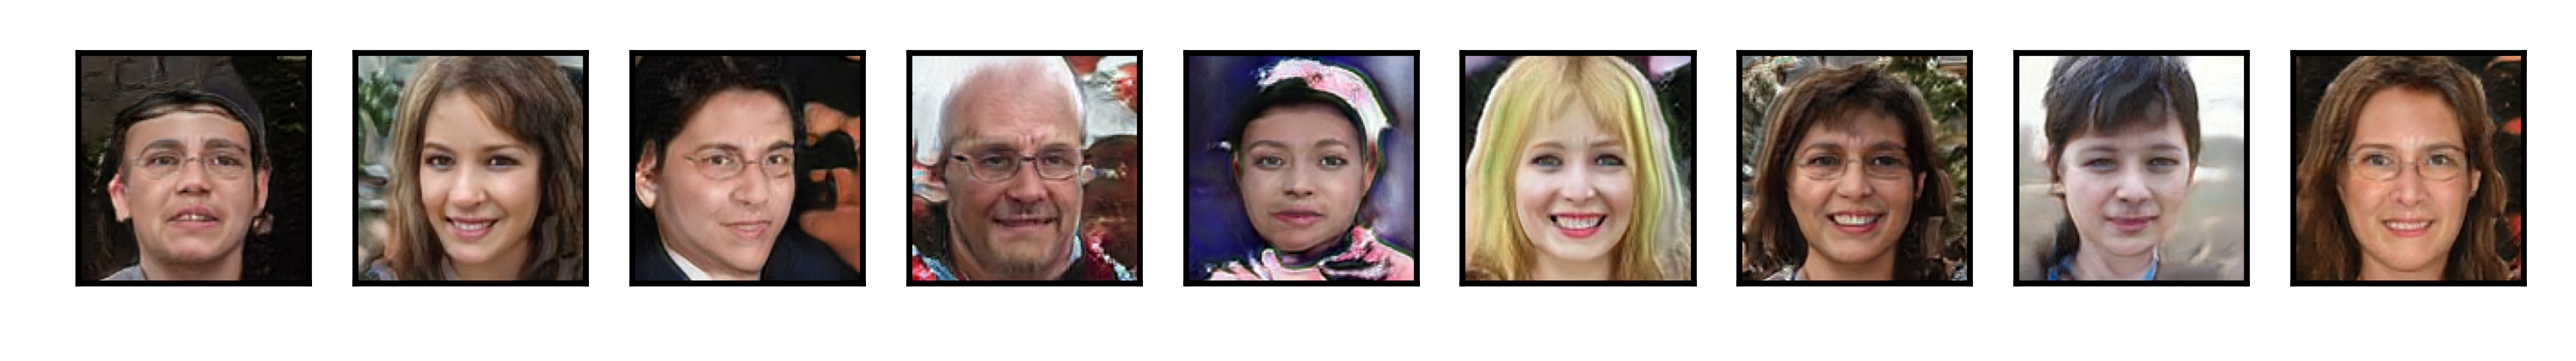
\includegraphics[width=\linewidth]{ffhq-random_Stylegan2.png}
		\vspace{-7mm}
		\caption{StyleGAN2.} 
	\end{subfigure}
	\begin{subfigure}{\linewidth}
%		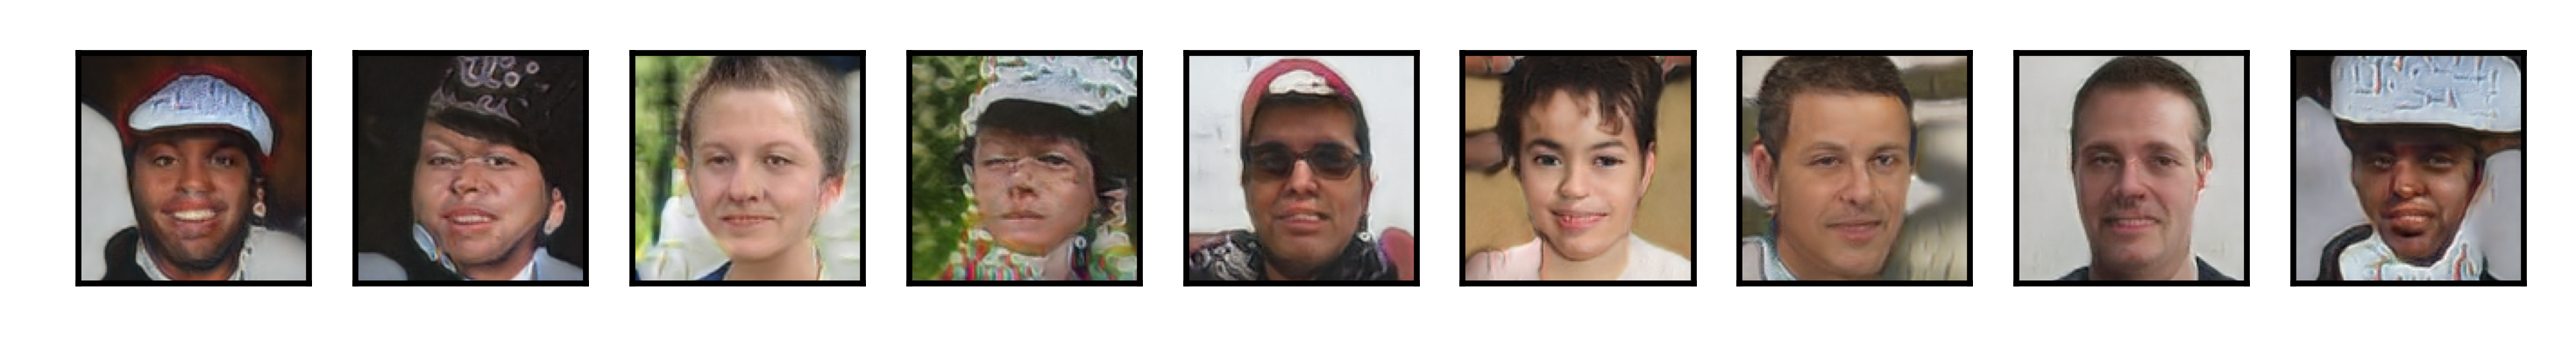
\includegraphics[width=\linewidth]{ffhq-random_GANFormerSimplexNoAtt.png}
		\vspace{-7mm}
		\caption{GANformer with Simplex attention and vanilla StyleGAN2 discriminator.}
	\end{subfigure}
	\begin{subfigure}{\linewidth}
		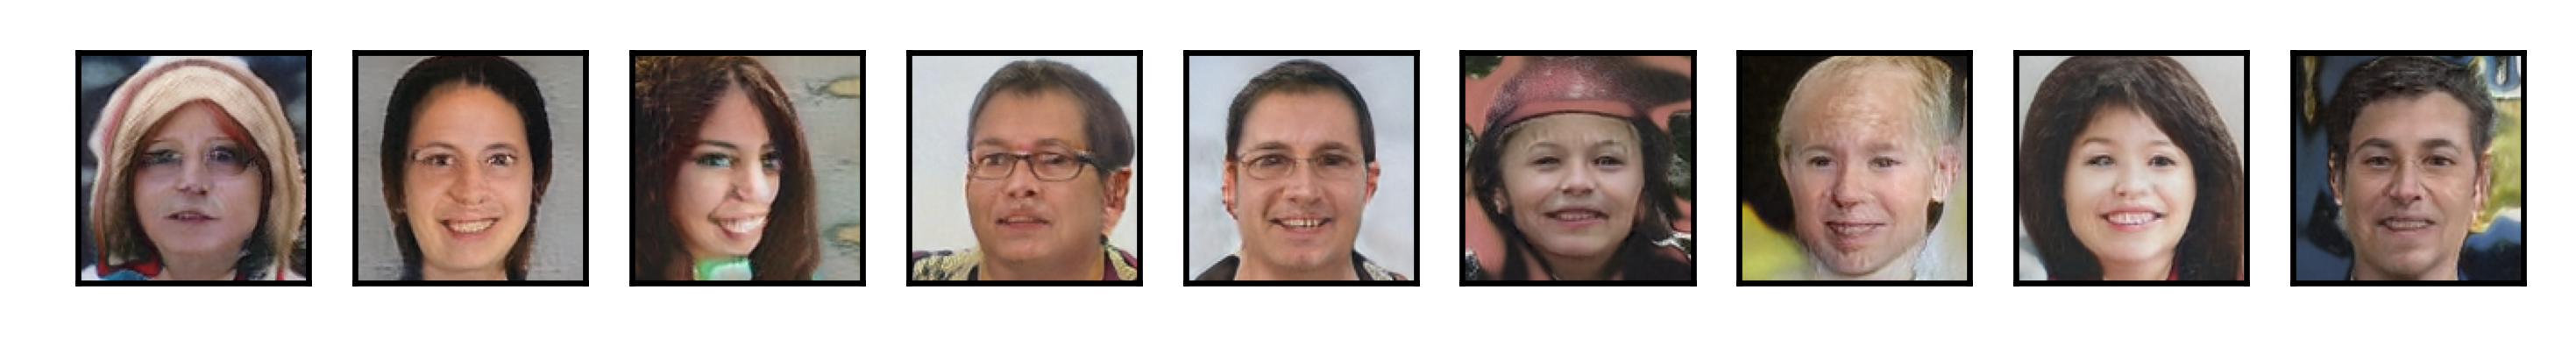
\includegraphics[width=\linewidth]{ffhq-random_GANFormerSimplexAtt.png}
		\vspace{-7mm}
		\caption{GANformer with Simplex attention.}
	\end{subfigure}
	\begin{subfigure}{\linewidth}
		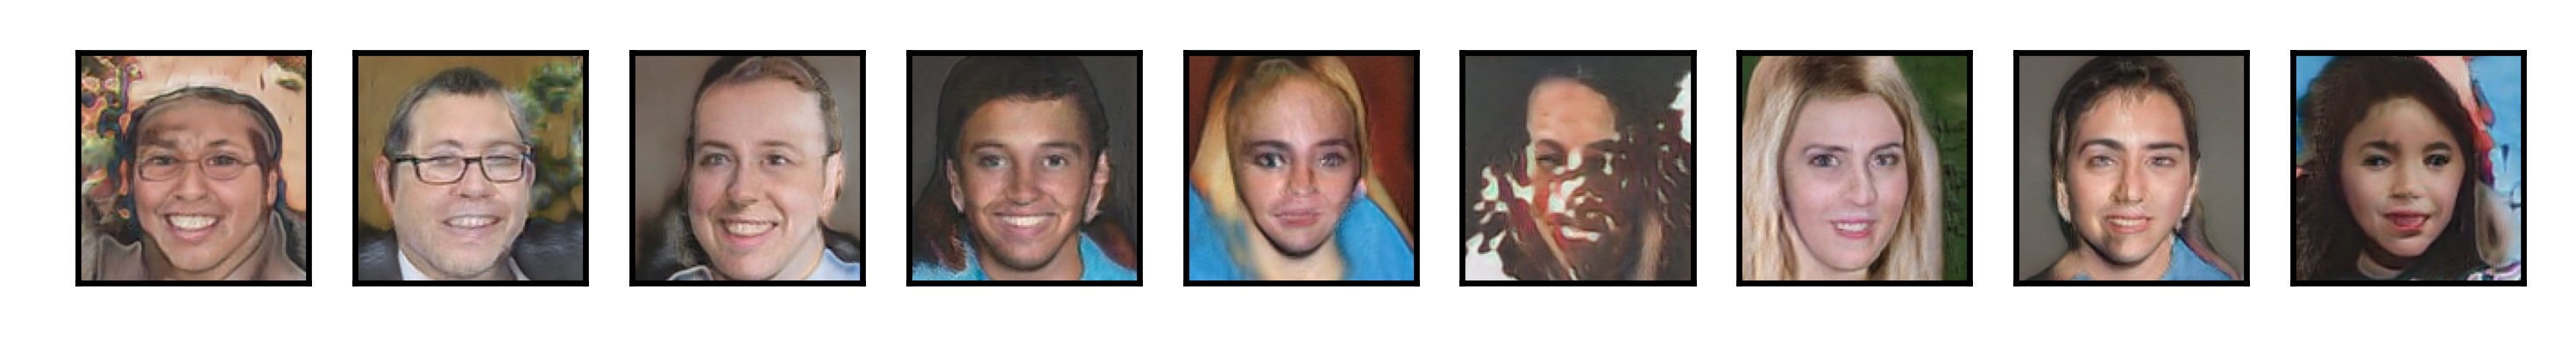
\includegraphics[width=\linewidth]{ffhq-random_GANFormerDuplexNoAtt.png}
		\vspace{-7mm}
		\caption{GANformer with Duplex attention and vanilla StyleGAN2 discriminator.}
	\end{subfigure}
	\begin{subfigure}{\linewidth}
		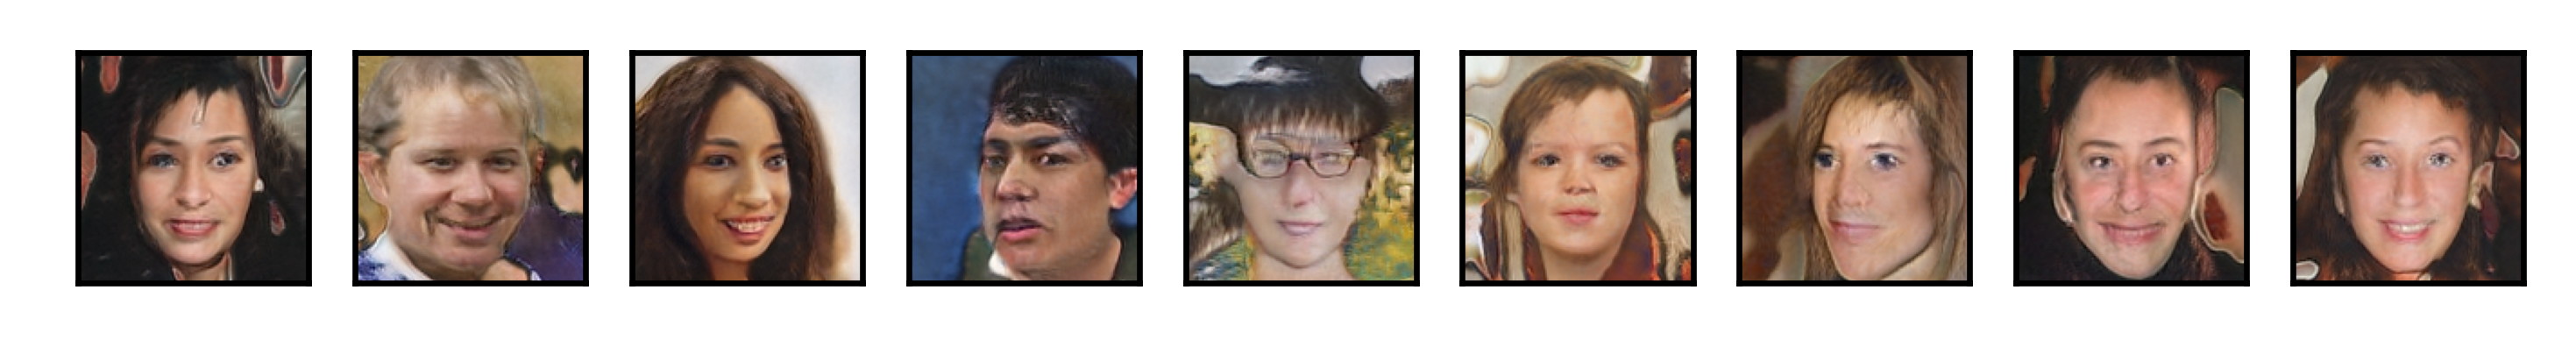
\includegraphics[width=\linewidth]{ffhq-random_GANFormerDuplexAtt.png}
		\vspace{-7mm}
		\caption{GANformer with Duplex attention.}
	\end{subfigure}
	\vspace{3mm}
	\caption{\textbf{Visualisation of 9 images generated with the various models}.}\label{fig:random-ffhq}
\end{figure}

\begin{figure}[htpb]
	\centering
	\begin{subfigure}{\linewidth}
		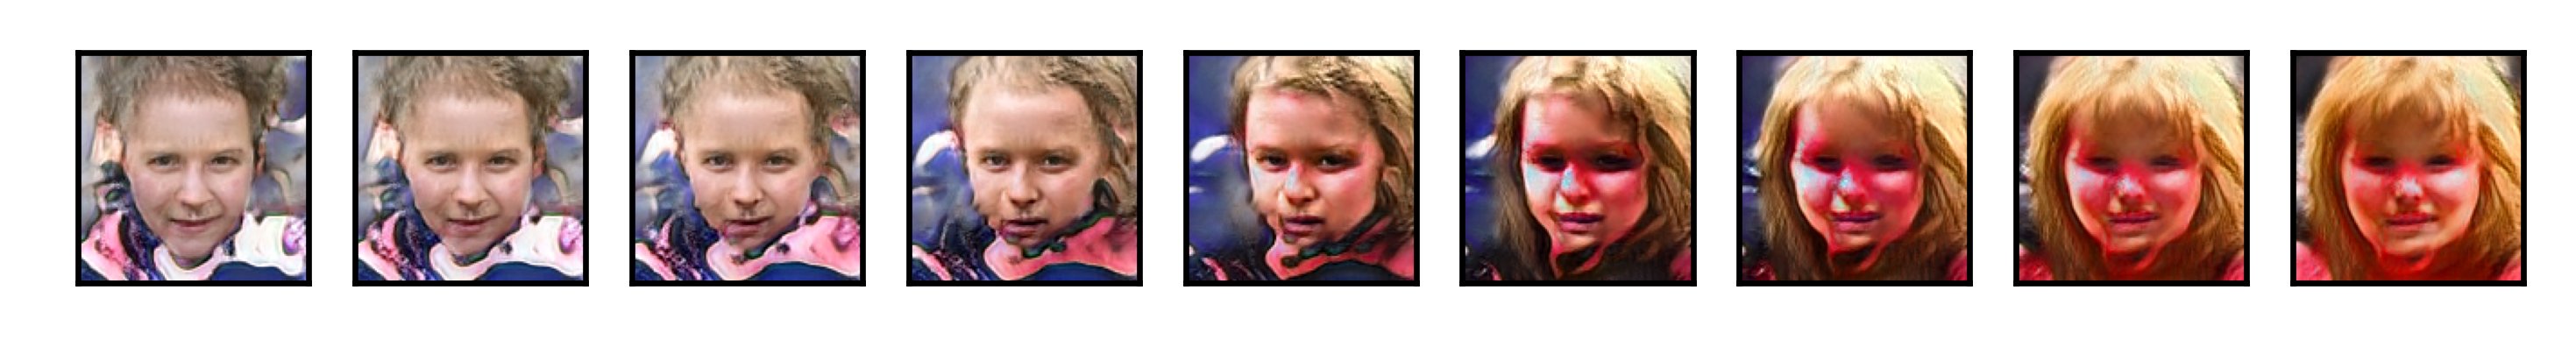
\includegraphics[width=\linewidth]{ffhq-interpolation_Stylegan2.png}
		\vspace{-7mm}
		\caption{StyleGAN2.} 
	\end{subfigure}
	\begin{subfigure}{\linewidth}
%		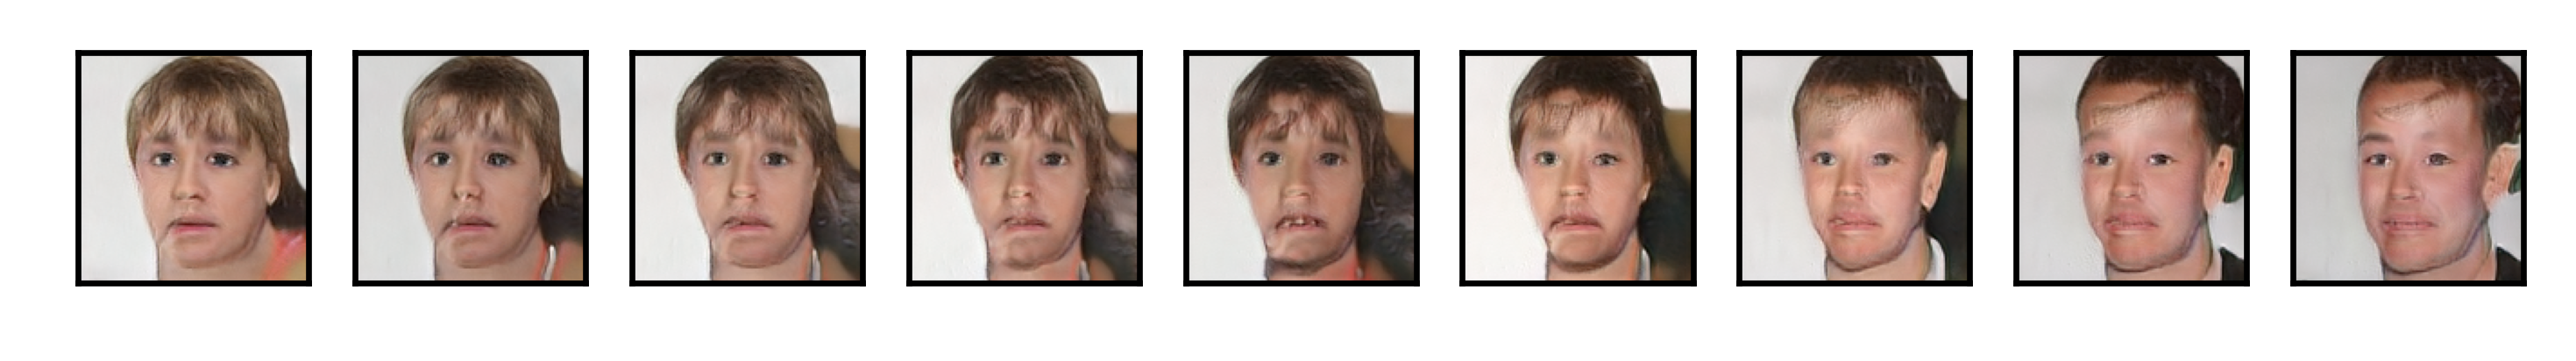
\includegraphics[width=\linewidth]{ffhq-interpolation_GANFormerSimplexNoAtt.png}
		\vspace{-7mm}
		\caption{GANformer with Simplex attention and vanilla StyleGAN2 discriminator.}
	\end{subfigure}
	\begin{subfigure}{\linewidth}
		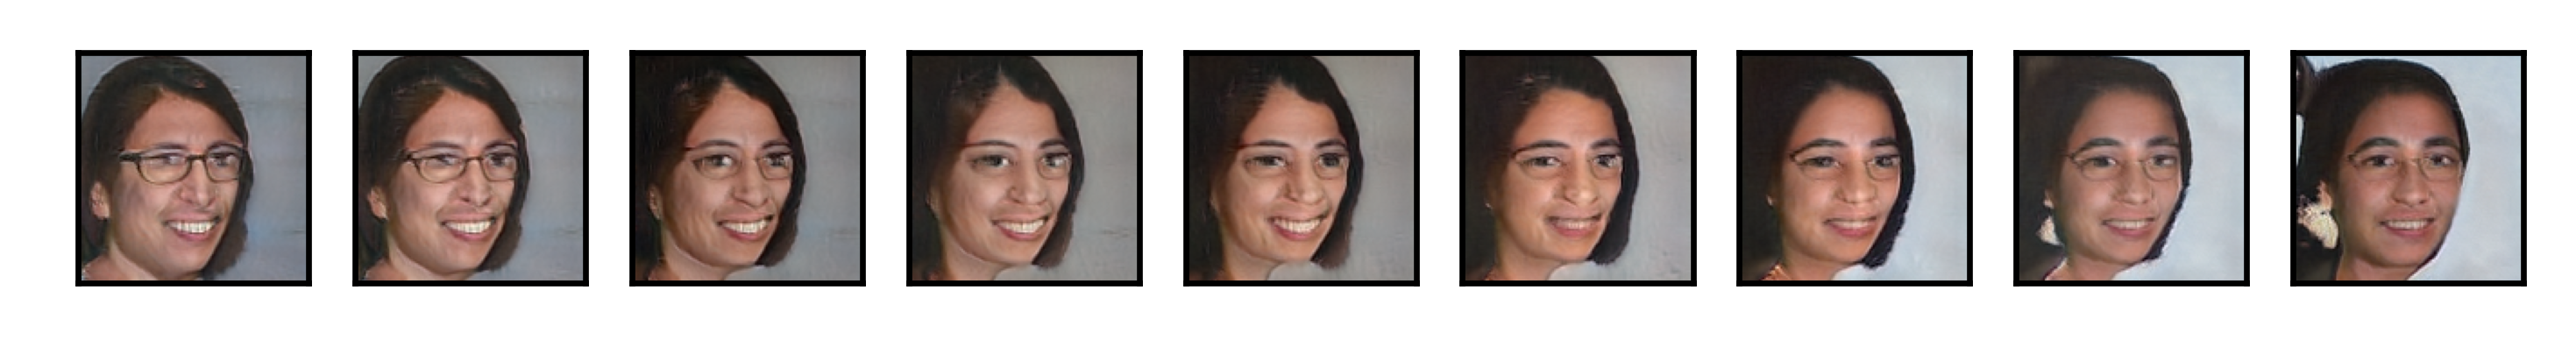
\includegraphics[width=\linewidth]{ffhq-interpolation_GANFormerSimplexAtt.png}
		\vspace{-7mm}
		\caption{GANformer with Simplex attention.}
	\end{subfigure}
	\begin{subfigure}{\linewidth}
		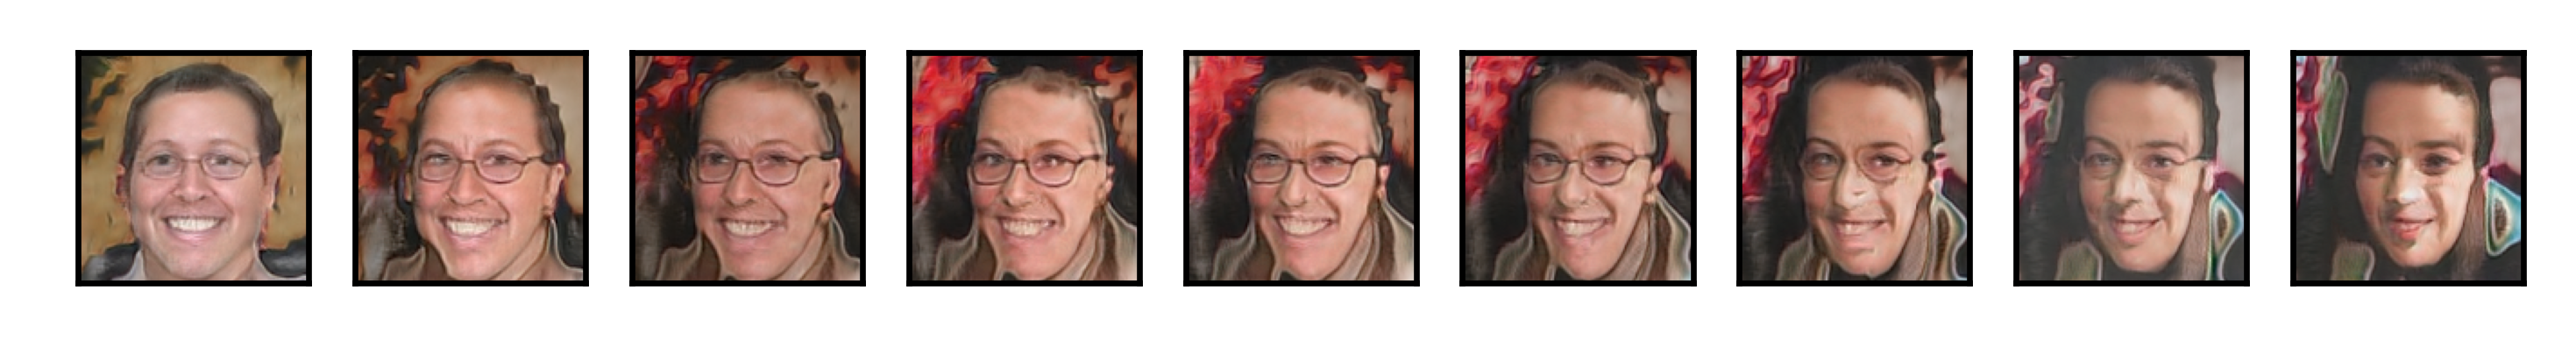
\includegraphics[width=\linewidth]{ffhq-interpolation_GANFormerDuplexNoAtt.png}
		\vspace{-7mm}
		\caption{GANformer with Duplex attention and vanilla StyleGAN2 discriminator.}
	\end{subfigure}
	\begin{subfigure}{\linewidth}
		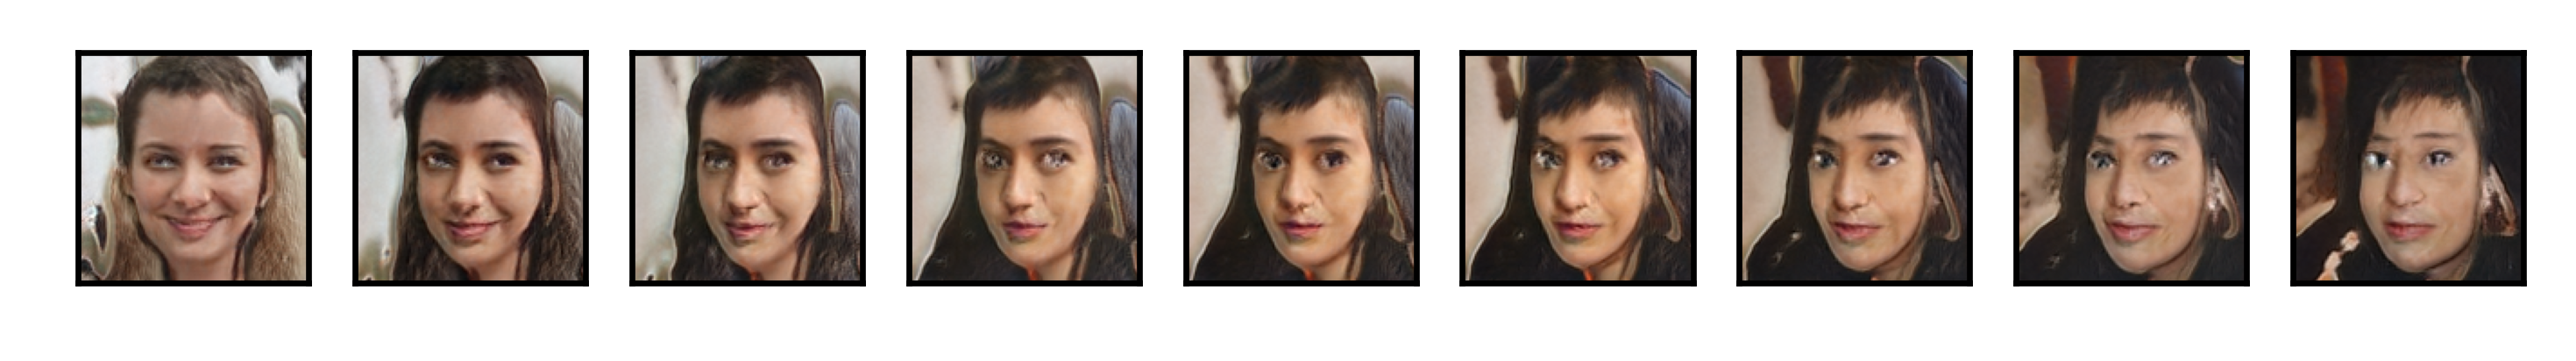
\includegraphics[width=\linewidth]{ffhq-interpolation_GANFormerDuplexAtt.png}
		\vspace{-7mm}
		\caption{GANformer with Duplex attention.}
	\end{subfigure}
	\vspace{3mm}
	\caption{\textbf{Simple $\mathbf{z}$ interpolation using of the various models}.} 
	\label{fig:interpolation-ffhq}
\end{figure}


\clearpage
\bibliography{bibliography}
\bibliographystyle{unsrtnat}
\clearpage

\end{document}
